\documentclass[11pt]{article}
\usepackage{graphicx}
\usepackage{caption}
\usepackage{chngcntr}
\usepackage[section]{placeins} % subsections
\usepackage[round, sort, numbers]{natbib}
\usepackage{makecell}
\usepackage{url}
\counterwithin{figure}{section}
\captionsetup[figure]{slc=off}
\usepackage[left=2cm, right=2cm, top=2cm, bottom=2cm]{geometry} % geometry of page
\setcitestyle{square} % square referencing style
\usepackage[fleqn]{amsmath} % for maths
\usepackage{subfig}
\setlength{\parindent}{0pt} % no indents on new paragraphs
\graphicspath{{Report/Figures/}}

\newcommand*\ruleline[1]{\par\noindent\raisebox{.8ex}{\makebox[\linewidth]{\hrulefill\hspace{1ex}\raisebox{-.8ex}{#1}\hspace{1ex}\hrulefill}}}

\usepackage{xcolor}
\definecolor{bookColor}{HTML}{232323}  % 0.90\% of black
\color{bookColor}

\begin{document}
\begin{titlepage}

    \begin{center}
        \vspace*{1cm}
        \Huge
        \textbf{Robotics} \\
        \vspace{0.5cm}
        \LARGE
        \vspace{1.5cm}
        \textbf{G. Sheppard, D. Thomas, J. Doering, J. Matthews, C. Li} \\
        \vfill
        \vspace{0.8cm}
        \Large
        University of Birmingham\\
        Physics and Astronomy Department\\
    \end{center}
\end{titlepage}

\tableofcontents

HERE IS A LIST OF WORDS THAT WE SHOULD CHECK AT THE END TO MAKE SURE WE HAVE ALL USED THE SAME

Double pendulum not triple pendulum \\
Nao not NAO (or other way let's just keep it constant)\\
Posture not position\\
Start-up not startup\\
Large encoder not big encoder (sounds better I think)\\
Rotational not torque\\
Centre point not zero point (as now swings through the centre etc)\\
Set-up not setup (probably this way round who knows tbh) ((They mean slightly different things i think))


\section{Abstract}
\cite{Bae2006}.

\section{Introduction}
\subsection{Background}
\subsection{Motivation}
\subsection{Theory}

\section{Connecting To Nao}

\subsection{Nao}
Initial connections to Nao performed using choreographe good to familiarise with joint names and connections (graph of joint names, limited by implementation, switched to using the ALProxy and created a joint name model to better understand the joint and connections

Can connect to both virtual and simulated robots in order to check motions before implementing 

Improved on positions from previous years to maximise each posture to extend as far as possible 

Increased the speed of NAOs kicks as previous years limiteted by using the set range of the knee pitch as there max angle as they  assumed this was the largest angle and so the one to maximise

instead based on the range of individual positions 

Put in stops to prevent the angle aching to far, same with checking the initial posture when setting up the postures

communicate directly using python scripts


Include diagram of joints and talk about connecting and extracting sensor values and calling joints using python dictionaries:
Normalising speeds, creating algorithms to ensure simultaneity.
Slowing initial speed of NAO to prevent injury during initialisation of positions.
Defining positions to ensure left and right side was symmetric and improved on previous years positions my maximising the range of motion with fail safes to ensure a correct position was reached by comparing joint data with expected position\\

Small amount about compatibility issues and that these were resolved by using the same python SDK and choreagraph versions and running code via linux to prevent issues with compiling and installing: 

Creating 

\subsection{Encoders}
\ruleline{George Sheppard}
There are two sets of hinge encoders used, the large/big encoder, and the small encoders. The large encoder records the angle from the vertical to the largest rod of the swing. The small encoders record the angle with respect to the previous rod, there are 2 on each side of the swing.\\

A large amount of time was invested into connecting to these hinge encoders from any computer other than the lab one. Unfortunately, due to the nature of the shared object files required by the encoders, the set up is complicated and it is advised to use the lab computer when using the hinge encoders.\\

A guide for setting up the hinge encoders is provided in the wiki found in \ref{sec:wiki}.

\subsection{Interface}\label{sec:Interface}
The creation of each individual algorithm required the use of a substantial amount of common code, such as the logic required for: connecting to Nao, collecting values from the hinge encoders and Nao, handling of previous collected values, switching Nao's position, and storage. For this reason an interface was created that functioned as a base that all algorithms were built off, the logic of this base code is illustrated in figure \ref{fig:InterfaceLogic}. The interface starts by collecting all values required for the algorithm decision making process, it then passes these values through the algorithm, depending on the output of the algorithm it will either change Nao's position, switch to the next algorithm, or finish and store the data. It also fixes the sample rate to a specified frequency.\\

    \begin{figure}[!htb]
        \centering
        \captionbox
             {The logic behind the interface, all that required changing was the algorithm logic that the decision making was based on.\label{fig:InterfaceLogic}}
             {\includegraphics[width=1.0\textwidth]{InterfaceLogic.eps}}
    \end{figure}

With this base structure in place, creating an algorithm involved one function that took a set of values, and decided how to react to them, the algorithm had access to all past data to help in decision making. As these algorithms were defined in the same way, it is easy to switch between different algorithms mid swing, such that the motion of Nao could be more stringently controlled. For example Nao could be told to increase to $30^o$, then maintain this amplitude for $10s$, and then finally decrease back down to $0^o$.\\

With this base structure in place, creating an algorithm had two requirements: it took the set of values given to it by the interface, and it returned either 'switch', None, or any of the named positions that were defined in the Robot subsection of the interface e.g. 'Seated', 'Extended' etc.\\

As the interface required the encoders and the robot to connect to, a series of mock classes were created that aimed to replicate their functionality. This meant that away from the lab these fake classes were used as a substitute for the real encoders such that the interface could be developed without errors.

\subsection{Testing}
One of the main advantages of this setup was the ability to test algorithms without connecting to either the robot or the hinge encoders. As all previous data collected in the lab were stored, a setup was developed that read the file in line by line and passed it through the algorithm. This is exactly what would happen in a real test except the real data is replaced with the pre-recorded data.\\
Properties such as the position of Nao at each cycle, and the current algorithm the interface was on is recorded in both the real mode and the testing mode. This meant how each algorithm reacted to different scenarios could be plotted away from the lab, given that pre-recorded data that mimicked that scenario existed.\\
One downside of this method was that the data being fed into the algorithm wasn't reactive to the previous decision of the algorithm, as all the data was pre-recorded. This meant that this method was in no way a full replacement for testing the limits of the algorithm in the lab, but instead was used as a way to check that the algorithm was logically correct before spending limited time with Nao on it.

\subsection{Optimisations}
As discussed in section \ref{sec:Interface}, the interface would record any data relevant to the motion of the swing and Nao. This data could be used to effectively diagnose any problems with the motion, or investigate any other properties of Nao that could be useful in creating new algorithms. This amount of data, however, became a performance issue in certain situations, and this section is dedicated to discussing the optimisations made regarding this.

\subsubsection{Small Encoders}
\ruleline{Jonathan Matthews}
One of the obvious sources of delay in the system is the set of small encoders attached to the swing. These encoders are incredibly useful in modelling the double pendulum of the swing, however, they are irrelevant when the swing is setup in it's simple pendulum mode with all the joints fixed. For these reason there were two setups created for the interface, one that recorded from both the large and small encoders, and one that only recorded from the large encoder only.\\

A method that was investigated to avoid this problem was the introduction of multiprocessing into the interface....
TODO: JONATHAN FINISH THIS BIT, WHY DOESN'T IT WORK, WHAT IS THE SAMPLE RATE OF THE SMALL ENCODERS

\subsubsection{Nao}
\ruleline{George Sheppard}
A second source of delay was the transmission of data to and from Nao. A small subset of this transmission data was paramount to the success of the algorithms, such as the commands for changing the joint positions. A large amount, however, were redundant in certain situations. An example of this was the accelerometer values, initially these were included such that algorithms could be created using only values collected from Nao. A large majority of the time, however, these values were not being used in the algorithms or even looked at when investigating problems with Nao etc.\\

For this reason when creating an algorithm the user could input flags that allowed them to define whether they required these values, when they didn't require these values then fake values would be returned such that performance would increase.\\

Once the optimisations to both the small encoders and the calls to Nao, the interface was able to sample at a maximum of around $200$Hz, and at this point the large encoder was restricting any further increases. For most algorithms, however, the workload required by the individual algorithm would restrict this sampling rate before this point. 

\section{Swinging}

\subsection{Webots} \label{sec:webots}
\ruleline{James Doering}
Webots is a program that can simulate robots in a virtual environment with accurate physics and sensory feedback. In the same way that the real Nao can be communicated with via the Python library NAOqi, the virtual Nao can be controlled via NAOqisim, which is available [PUT STUFF HERE]. Through this method, Python code can be run through the NAOqi library, and sent to the NAOqisim controller in Webots, meaning that code can be tested away from the lab. This was especially useful for defining Nao's postures, as described in figure \ref{fig:webotspostures}. Webots automatically calculates the centre of mass of Nao - by removing the floor and setting gravity to be 0, the centre of mass relative to Nao's accelerometers could be found for each posture. This allowed for the 'raised' and 'lowered' postures to have the largest possible difference in heights for the centre of mass, optimising the parametric motion.\\

Webots also offered semi-accurate physics simulations, with some caveats. Using the swing modelled by the previous year revealed that the virtual Nao will easily assume it is falling, activating its fall manager and changing the algorithm's current posture. If the computer running Webots was weaker, the simulation would quickly become physically inaccurate and the algorithm would desynchronise. Finally, Webots offered no simple way of extracting the hinge encoder data in real time - this forms the basis of most algorithms, and so it could only be used for very simple tests. More information on setting up Webots can be seen in [PLACE REF HERE]

\textbf{I WILL REWRITE AND ADD IN FIGURES}

\begin{figure}
    \centering
    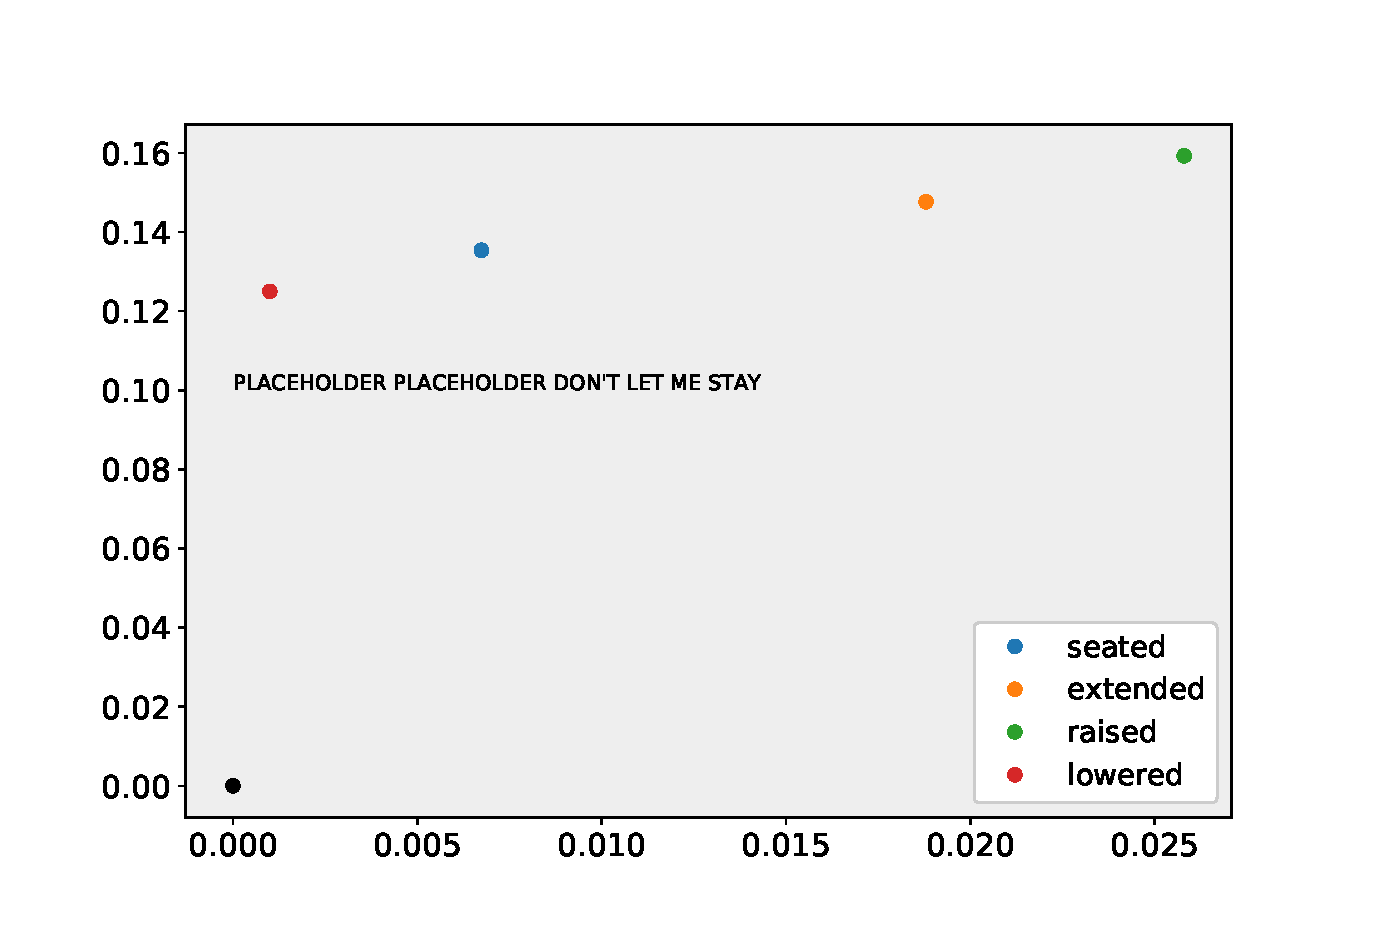
\includegraphics[width=0.6\linewidth]{COMPLACEHOLDER.eps}
    \caption{PLACEHOLDER: Will eventually show a nice comparison of Nao's centre of mass in each posture.}
    \label{fig:centreofmasses}
\end{figure}

\begin{figure}
    \centering
    \includegraphics[width=0.5\linewidth]{}
    \caption{PLACEHOLDER: Will have all 4 postures}
    \label{fig:postures}
\end{figure}




\subsection{Optimising Nao's Kicks}
\ruleline{David Thomas}

\subsection{Rotational Method}
\ruleline{David Thomas}
\begin{align}
    &\frac{\Delta E}{E} = 1 - e^{\frac{-2\pi}{Q}}\\
    &\text{At maximum angle},\\
    &E = lmg(1-cos(\theta))\\
    &\Delta E = E(\theta_a) - E(\theta_b)\\
    &\theta_a = \theta_b + d\theta\\
    &\frac{d\theta}{dt} = c - \frac{1-e^{\frac{-2\pi}{Q}}}{dt}\frac{\theta_b}{2}, \, \text{for small angles}
\end{align}
David: Say used previous defined positions, different methods for each algorithm (quarter period, integreation of theory team calculation of max angle), results for each, try to fit maximum amplitude peaks to linear to see if proportional to distance rocked or not, how results varied on different parameters such as if he swings before peak, during, or after, limitations to each method.
Calculations of offset parameters to maximise amplitude gain and comparison of each plot

\subsection{Parametric Method}
Jon: Talk about using the two extra positions defined for this motion from david, the idea behind the algorithm, results try to fit to exponential curve to see if it multiplies amplitude by fixed fraction like worksheet showed, any limitations, were two positions just different in vertical centre of mass or did horizontal distance change too

\begin{align}
    &\theta_a = \theta_b (\frac{L_{squat}}{L_{stand}})^{3/2}\\
    &\theta_a = \theta_b + \frac{d\theta}{dt}dt\\
    &\theta_b + \frac{d\theta}{dt}dt = \theta_b (\frac{L_{squat}}{L_{stand}})^{3/2}\\
    &\frac{d\theta}{dt} = \frac{\theta_b}{dt} ((\frac{L_{squat}}{L_{stand}})^{3/2} - 1)\\ 
\end{align}


\subsection{Damping}
\ruleline{James Doering}
\textit{I'm putting a general section on the damping each posture produces, how it was found, and a comparison of how the expected motion would look with and without damping. This is all basic skeleton text right now, will rewrite in the coming days.}

The combined damping of the swing can be modelled as an exponential decay of amplitude, modelled as 
\begin{equation} \label{eq:damping}
    \theta = \theta_0 e^{-bt}.
\end{equation}
By taking data of the swing being released at $\approx 10^\circ$ and fitting the decay of amplitude to a curve following equation \ref{eq:damping}, the coefficient of damping $b$ can be found. The results for this method can be seen in figure \ref{fig:dampingpositions}. The full values and method of fitting can be seen in section \ref{sec:dampingboring}.

    \begin{figure}[]
        \centering
        \captionbox
             {The swing's damping fitted for each posture described in section \ref{sec:webots}.\label{fig:dampingpositions}}
             {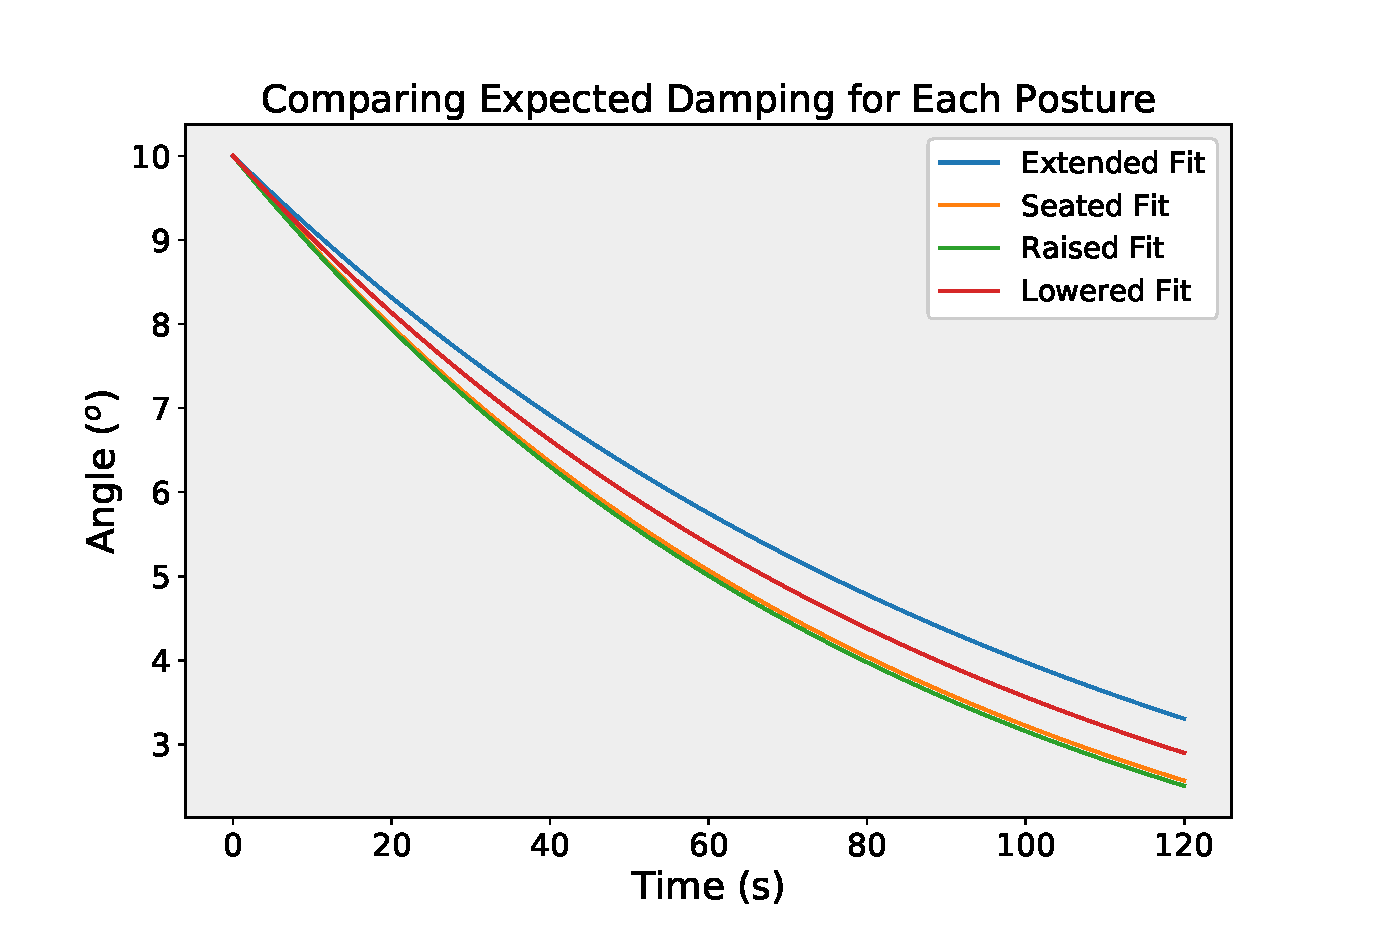
\includegraphics[width=0.7\textwidth]{DampingComparison.eps}}
    \end{figure}
 
From this figure it can be seen that the "seated" and "raised" postures produce the most damping, and the "extended" causes the least - this is likely due to air resistance blah blah George might discuss this.\\

This model of damping can be used as an alternative way to estimate the maximum angles will produce. From section [REFER TO THEORY SECTION] the rotational method is expected to produce a linear increase in amplitude per cycle. By combining this linear growth with the exponential decay, and solving the differential equation, we find that the rotational method can be modelled as
\begin{equation}
    \theta = \frac{m}{b}\big(1-e^{-bt}\big),
\end{equation}
where $m$ is the rate of change of amplitude expected for the rotational method and $b$ is the coefficient found through equation \ref{eq:damping}. By measuring the linear growth using the rotational quarter period algorithm in section [REFERENCE A SECTION, NEEDS RECONSIDERATION] to find m, the plot in figure [REFERENCE FIGURE] was produced.\\


[FIGURE HERE]

This shows the expected maximum amplitude........


\ruleline{George Sheppard}
I'll talk about how much of the damping comes from the air resistance and how much comes from the bearing torque friction, then may calculate the maximum theoretical angle Nao should reach


\section{Single Pendulum}
\subsection{Start-up}
\ruleline{James Doering}
There are multiple different ways to begin a swing from rest, the most intuitive being to "kick off" from the ground - due to Nao's short legs, this was not achievable.This was solved in previous attempts by using a weighted box to kick away from, or by manually pushing Nao, giving the initial amplitude required for normal swinging to be effective. In order to achieve our goals of a fully self-sufficient swinger, a dedicated start-up algorithm was developed. The method is simple - Nao kicks into the extended posture, waits a quarter period, kicks into seated, and then loops between waiting a half period and kicking into the next posture. The initial quarter period wait is used to account for Nao beginning in the centre of his swing, not at the edge. \\



As can be seen in figure \ref{fig:startup}, this method is blah blah blah... The period was calculated from previous data of nao swinging blah blah... noteably, the period of the swing changes slightly depending on the posture, but this was not considered in the code due to the difference in timing being miniscule... \\

This script also offers a good comparison for mass vs no mass etc etc etc etc etc etc etc...


\subsection{Timing Maximas}
\ruleline{George Sheppard}
To create algorithms that are efficient at applying Nao's energy into the motion of the swing requires an accurate estimate of the maximum angle of the swing, or the time at which this occurs. To early a swing dissipates the energy, and too late doesn't take advantage of the boost in velocity caused by changing position. For this reason a discussion of the best method for determining the maximum of the swing is outlined in the sections below.

\subsubsection{Timing via Angular Velocity}
\ruleline{Chenglong Li}
The angular velocity algorithms is developed base on the fact that the sign of the angular velocity will change just after the Nao hits its maxima. Therefore one can instruct the Nao to change its posture whenever the angular velocity change its sign. This algorithm is very easy to implement since there is no calculation involved and very reliable. Because Nao will never miss any kicks. However, there are two serious weakness for this algorithm. 
\\
\\
The first one is that this algorithm do not learn from old data, because this algorithm use the instantaneous big encoder value to decide if Nao should kick or not. This indicates that the angular velocity method does not have the ability to improve itself. The second weakness of this algorithm is that one cannot set offset in this algorithm. Assuming that an algorithm predict that Nao should be at the maxima at time T or angle A but one would like Nao to kick a little bit earlier or latter. Hence one can set Nao to kick at T + offset or A + offset. The offset can be positive or negative. However, due to the nature of the angular velocity algorithm, Nao will only know it is at the maxima after it passed the maxima. Therefore it is impossible to set offset for this algorithm. 

\subsubsection{Timing via Maximum Angle}
The max angle algorithm uses the energy conservation law to predicts the next possible max angle that Nao can reach. Two different algorithms are developed. The first one is using the simplest energy conservation law in simple pendulum assuming there is no damping involved The equations are shown below:

\begin{align}
    &\frac{1}{2}MV_{max}^2 = Mgh\\
    & h = \frac{V_{max}^2}{2g}
\end{align}

The $V_{max}$ is the maximum speed that the swing reached in every cycle, which is observed at the minima and h is the difference in height between the minima and the next maxima. To record the max speed at bottom, One should record the two big encoder data that the sign of the big encoder value just flipped. However, it is very inaccurate to just use the big encoder value just before or after the minima because the max speed is affected highly when only two data point was used. Hence one have defined the max speed is the average speed that from -1 to 1 degree.
\\
\\

Once the height difference is determined, one can calculate the next maximum angle by using the technique shown in figure \ref{fig:max_angle_calculation}

    \begin{figure}[!htb]
        \centering
        \captionbox
             {Illustration of using height difference h and pendulum length L to calculate the max angle $\theta$\label{fig:max_angle_calculation}}
             {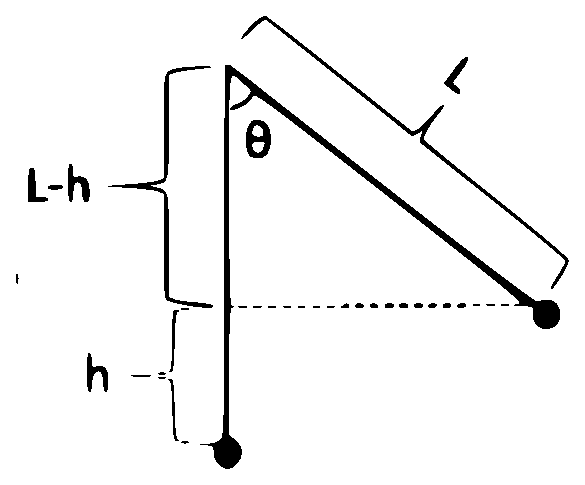
\includegraphics[scale = 0.85]{max_angle_calculation.eps}}
    \end{figure}
    
Now one could calculate the max angle $\theta$ using:
\begin{align}
    &\theta = cos^{-1}(\frac{L-h}{L})
\end{align}





\subsubsection{Timing via Quarter Period}
\ruleline{George Sheppard}
The quarter period algorithm uses the time that the last quarter period of the cycle took to predict the time of the next maximum, and utilizes the fact that Nao's motion only increases in angle by a small amount per cycle. Whenever Nao swings through the centre of the swing, the first thing to calculate is an estimate of the time that Nao actually crossed the boundary. This is important as Nao swings the fastest through the centre, and therefore the first time recorded after he crossed may not be close enough to the true time. Shown in figure \ref{fig:InterpolationDiagram} is a diagram of this situation. 

    \begin{figure}[!htb]
        \centering
        \captionbox
             {Illustration of the values of the swing, before and after the crossing point.\label{fig:InterpolationDiagram}}
             {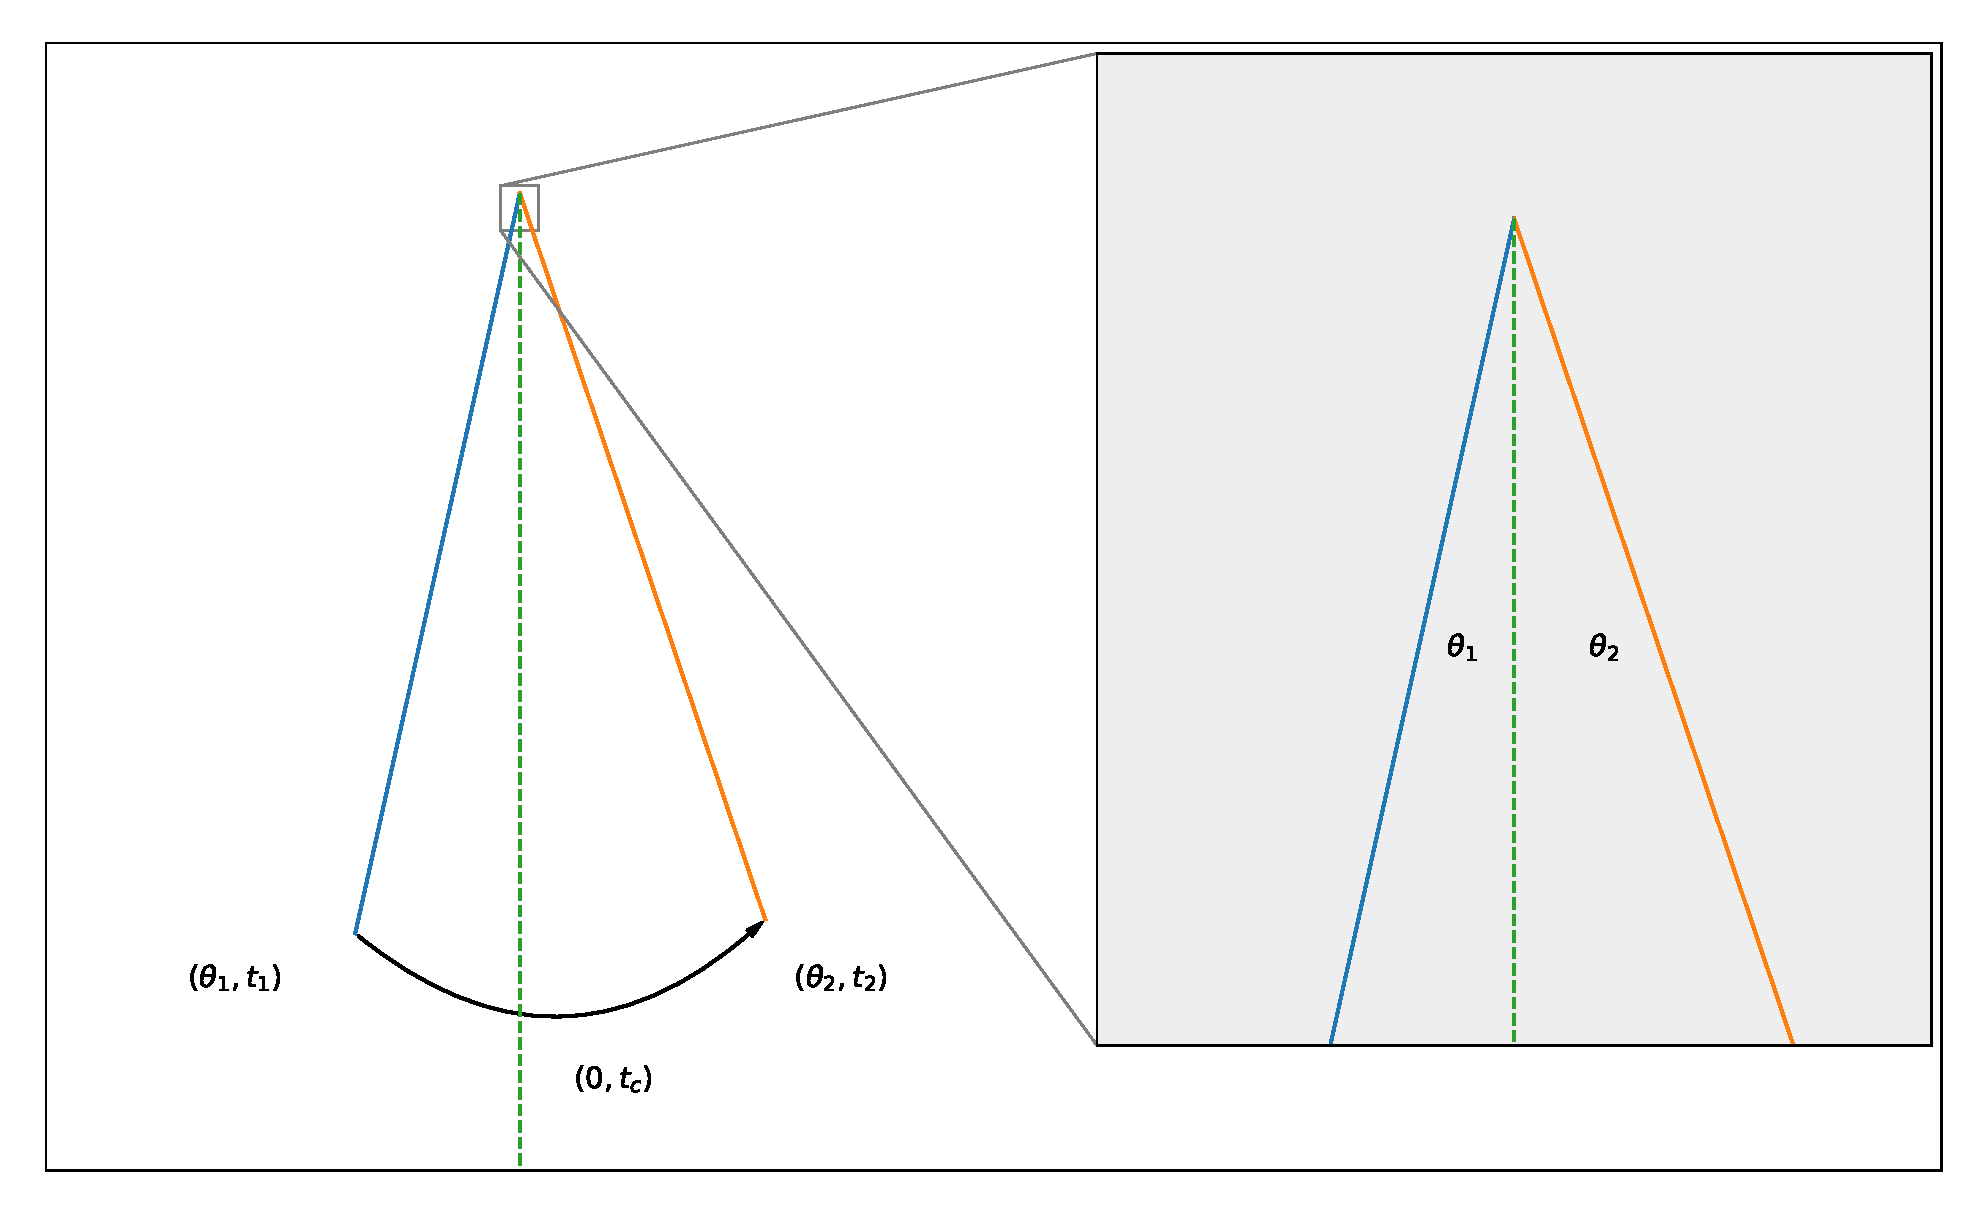
\includegraphics[width=1.0\textwidth]{InterpolationDiagram.eps}}
    \end{figure}

For angle and time $(\theta_1, t_1)$ before the crossing, and $(\theta_2, t_2)$ after the crossing, a linear interpolation can be applied to give a more accurate estimate of the true zero point crossing. This is calculated using

\begin{equation}
    t_c = t_2 - (t_2 - t_1) \frac{|\theta_2|}{|\theta_2 - \theta_1|}.
\end{equation}

As is expected for a higher sampling time this error on the true centre time is smaller. The second value to calculate is the time at which Nao was at the last angle maxima. This can be done simply as all previous values of the encoder are recorded. One small complication is the introduction of local maximas, these occur more often at low amplitude swings due to the jolted motion of Nao's movement, and need to be filtered out to allow a better estimate for the maximum angle time. To filter these local maxima out the moving average of the encoder values is calculated, this smooths the data, figure \ref{fig:MovingAverageDiagram} shows a comparison between the moving average of some example data, for this example the latest local maximum would be the calculated max time, but after using the moving average the estimate is much closer to it's true point. Using the modified encoder values the time of the maximum can be determined, and therefore the quarter period of the swing can be calculated. \\

    \begin{figure}[!htb]
        \centering
        \captionbox
             {Comparison of angle data before and after a moving average is applied.\label{fig:MovingAverageDiagram}}
             {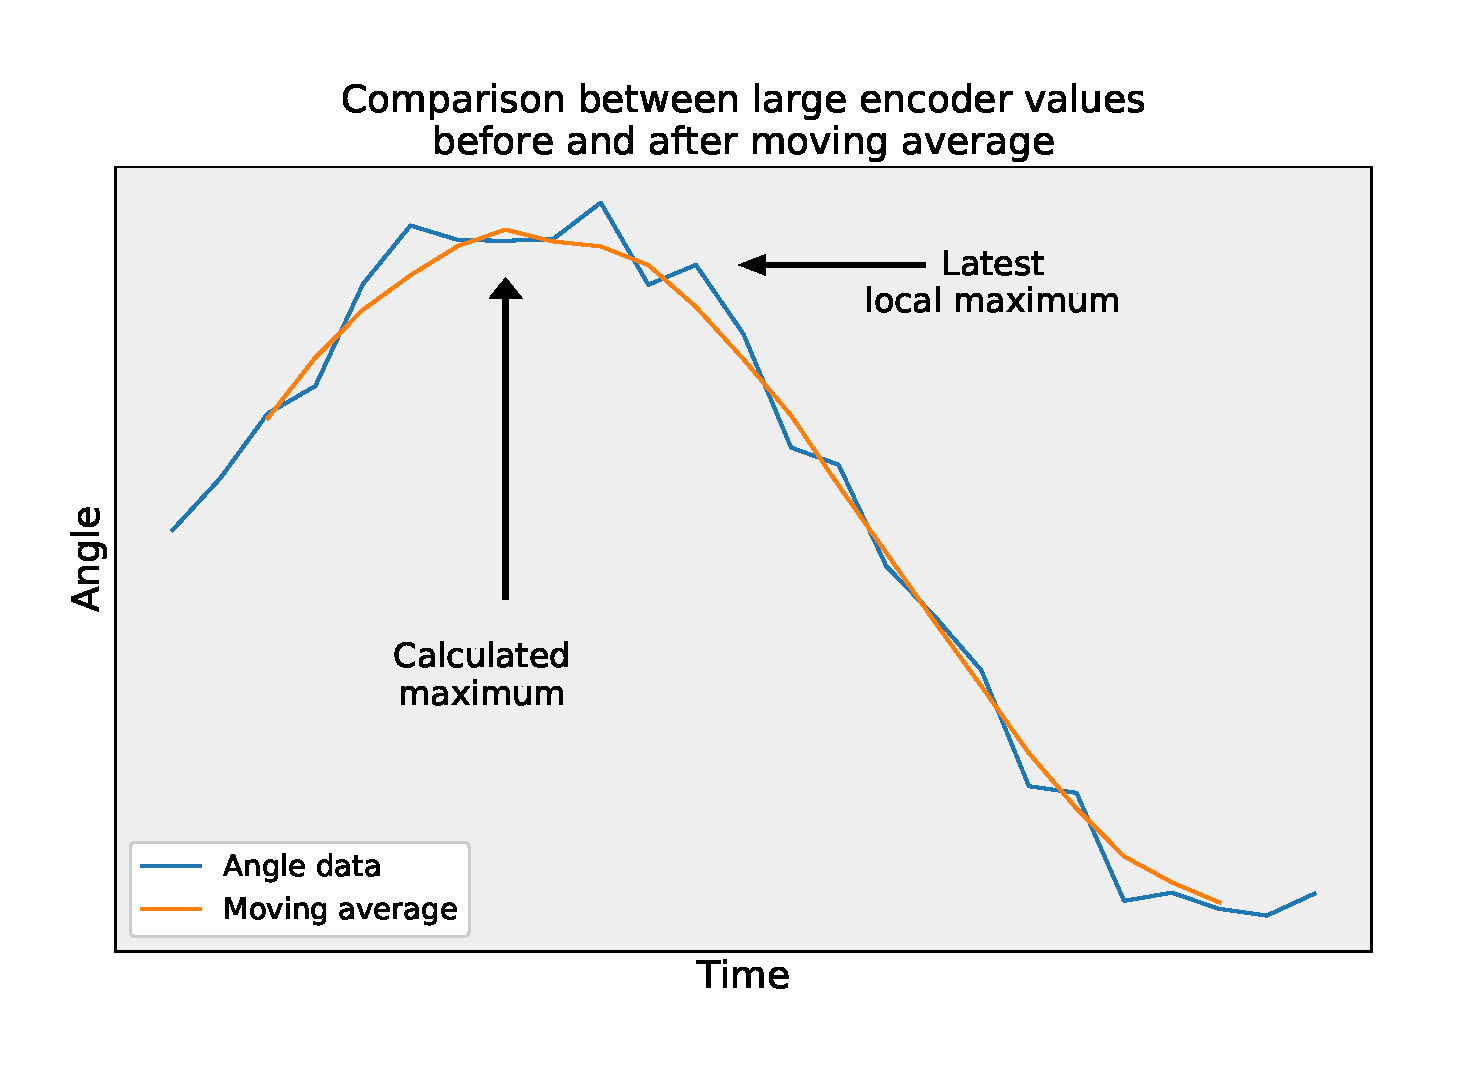
\includegraphics[width=1.0\textwidth]{MovingAverageDiagram.eps}}
    \end{figure}


This process is repeated every half period, whenever Nao crosses the centre point, such that the next maxima time can be calculated before it is reached. An advantage of this algorithm is that the estimate of the period is constantly updated, such that the calculation of the maxima time remains accurate for all amplitudes (as long as there is sufficient build up time to calculate the previous period). From here the only decision that needs to be made is whether it is better to swing before the maxima, at the maxima, or after the maxima, for the greatest amplitude swing.


\subsection{Investigation of Offest Values}
\ruleline{David Thomas}

\subsection{Increasing QP Rotational}\label{sec:Increasing QP Rotational}
\subsection{Increasing QP Parametric}
\subsection{Maintaining}
\ruleline{George Sheppard}
For Nao to be able to maintain his angle of swing requires the matching of the energy lost to damping, with the energy gained from his motion. This can be done easily for one specific angle by determining the correct time to kick to match this energy loss, however, for a generalised algorithm that is required to maintain at any angle requires a different method.\\

The first method for accomplishing this requires the use of a feedback loop. First, the angle that needs to be maintained is defined, and an offset is defined that is a guess at the correct time before/after the peak to create sustained motion. Nao is then left to kick using this initial offset, and by recording the angle of the maximas this offset can be adjusted to bring Nao closer to the correct amplitude. This offset can also be defined as the number of degrees before the maintaining angle Nao should kick at, such that the motion is maintained.\\

An alternative method for maintaining amplitude requires the use of a 'good', 'average', and 'bad' kick. Then when the angle increases past a critical point a bad kick can be used to decrease the amplitude, and vice versa for when the angle is lower than needed. The average kick is defined such that it is as close to a maintaining kick as possible, however, as this is not perfect the good and bad kicks compensate for it.

These three methods of maintaining are compared in figure \ref{fig:MaintainFeedbackComparison}, TODO: RETAKE THIS DATA AT 7.5 DEGREES AND ADD IN LINE FROM OLD JOE PLOT TOO\\

    \begin{figure}[!htb]
        \centering
        \captionbox
             {Comparison between using timed feedback and feedback based on angle for maintaining a $10^o$ amplitude swing.\label{fig:MaintainFeedbackComparison}}
             {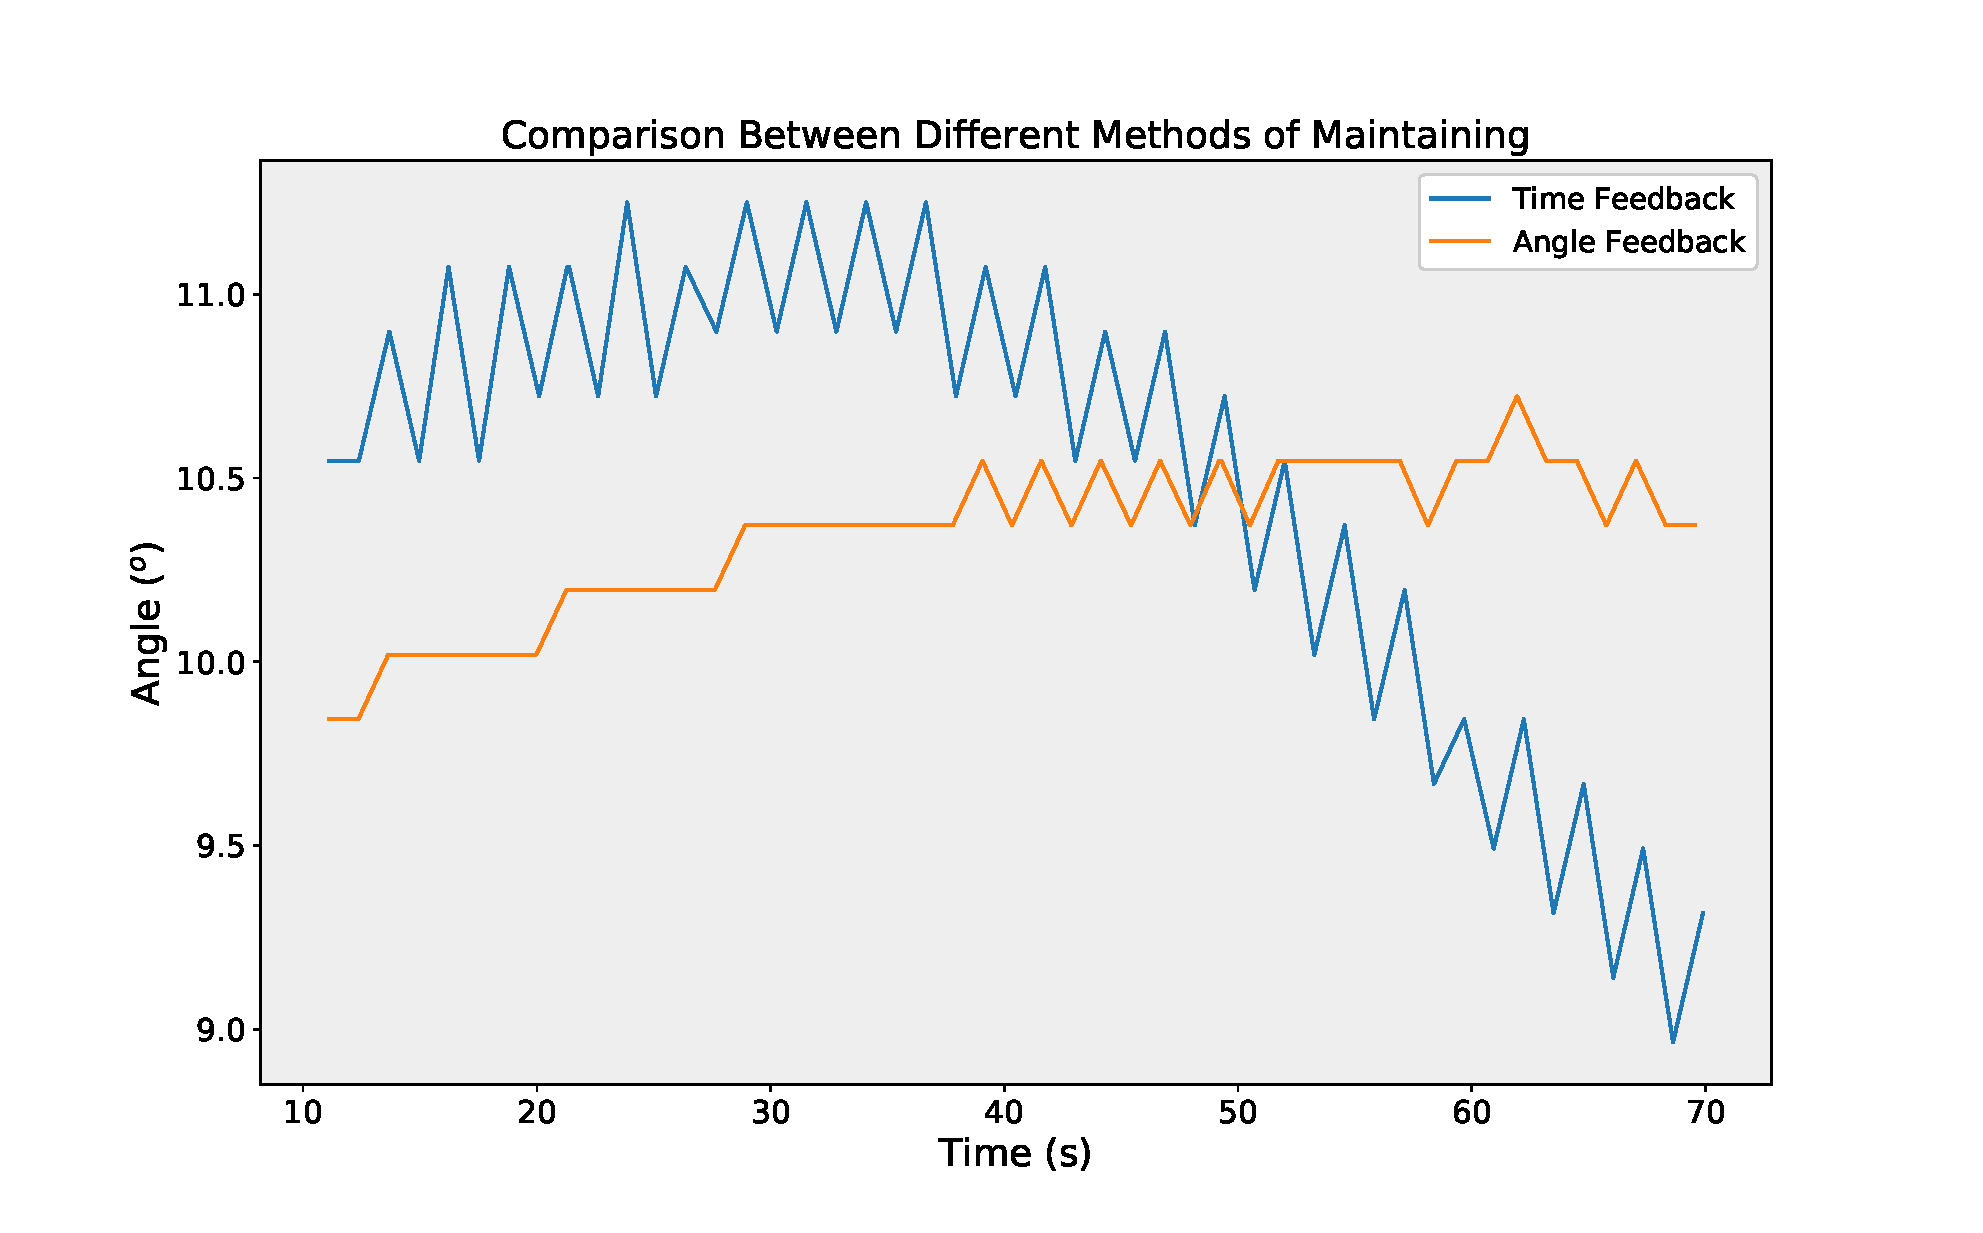
\includegraphics[width=1.0\textwidth]{MaintainFeedback.eps}}
    \end{figure}
    
TODO: DISCUSSION OF RESULTS\\
TODO: WHICH IS BEST WHICH IS WORSE, WHY IS THIS\\
TODO: DO ALL ALGORITHMS WORK FOR EACH ANGLE OR ARE THEY SPECIFIC TO CERTAIN ANGLES\\

\clearpage

\subsection{Decreasing}

\subsection{Using Accelerometer Values}
\ruleline{George Sheppard}
Nao's ability to swing in each previous timing method requires the use of external inputs, such as the hinge encoders. For Nao to truly swing unassisted an equivalent to the large encoder angle needed to be extracted from Nao's outputs only. It was decided that the accelerometer values, and more specifically the vertical accelerometer (Nao's Z accelerometer) would allow us to extract a sinusodial curve.\\

A comparison between the Z accelerometer data for both a static and changing posture during swinging is shown in figure \ref{fig:AccelerometerComparison}, this confirms that the Z accelerometer is the vertical direction, as for a static posture the accelerometer reading is of the order of $g$. It is sinusodial due to the sinusodial motion of the swing, and can be used to extract the maximas of the swing in the same way the large encoder is used, it is clear that the accelerometer frequency here is twice the frequency of the swing, as acceleration is maximum at both edges of the swinging motion. The introduction of a changing posture, however, causes the Z accelerometer to transition to something that resembles more of a square wave, and to be able to extract the maximas this data needed to be filtered, another interesting property that arises from switching posture is that the frequency is reduced to that of the swing, as the acceleration due to the swing is very small compared to the acceleration caused by changing posture.\\

    \begin{figure}[!htb]
        \centering
        \captionbox
             {Z accelerometer readings for a static posture and a changing posture.\label{fig:AccelerometerComparison}}
             {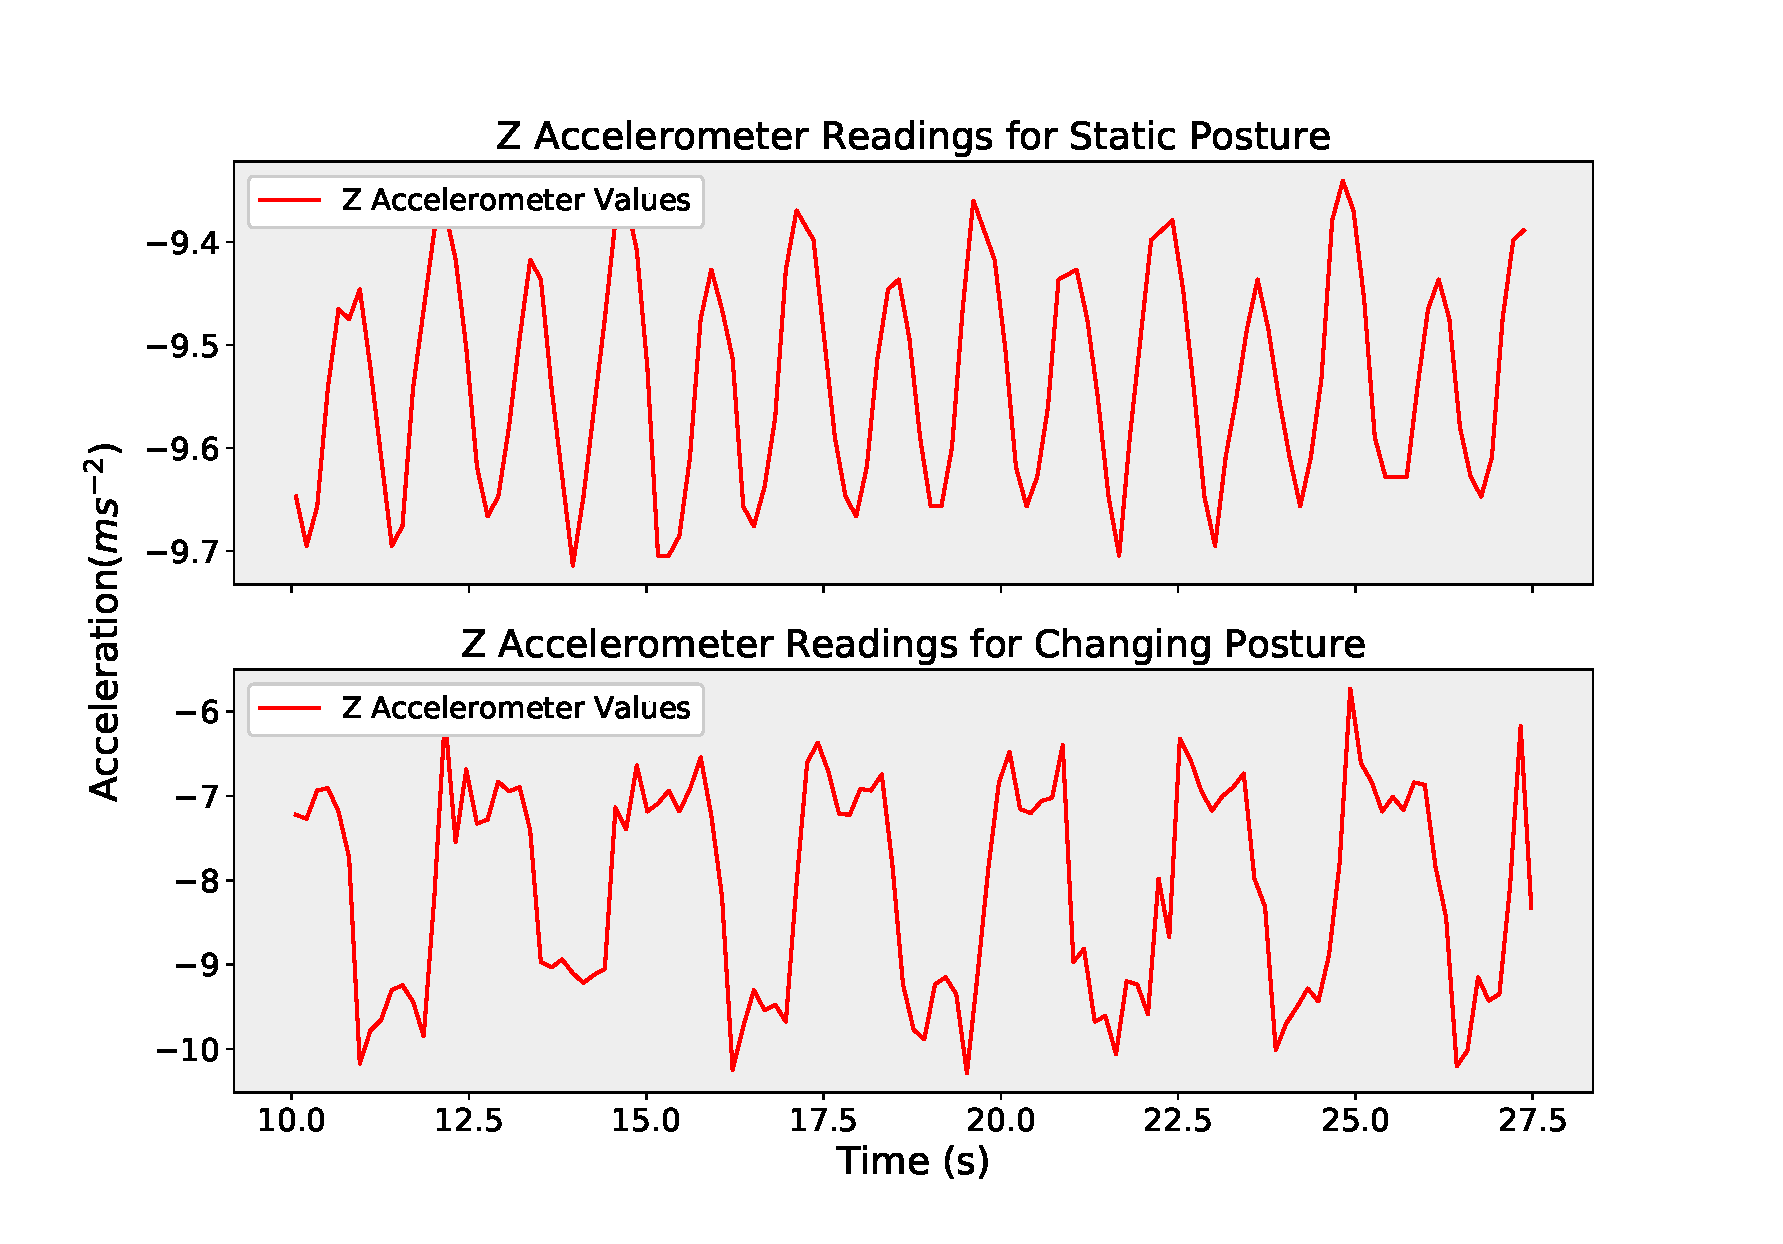
\includegraphics[width=1.0\textwidth]{AccelerometerComparison.eps}}
    \end{figure}

Figure \ref{fig:FrequencyDecomposition} shows a comparison between the frequencies present in the accelerometer data for a static posture, and for a switching posture, each dataset has been normalised by largest frequency peak. For the static posture dataset there are two spikes, the largest of which with a frequency of $0.8$Hz. This frequency is twice that of the swing, as the acceleration goes from maximum at the edge, to minimum at the centre point, back to maximum at the other edge. The other peak has a frequency of $0.4$Hz, this arises due to the asymmetry in Nao's seated position, as Nao's seated posture is slightly behind the seat, the maximum angle that he reaches will be asymmetric and will oscillate slightly higher and lower dependent on which side of the centre point he is on, this explains why it is at the frequency of the swing. To understand the frequency composition for the changing posture, it is worth looking at modelling Nao's motion. Nao's motion switches once at each maxima, and the switch point can be approximated as instantaneous, in other words Nao's motion is a square wave with the same frequency as the swing. The fourier transform for a square wave is

\begin{equation}
    f(t) = \frac{4}{\pi}\sum_{n=1}^{\infty} \frac{1}{2n-1}\sin(2(2n-1)\pi ft),
\end{equation}
where $f$ is the frequency of the swing, this means that there should be diminishing peaks expected at $0.4$Hz, $1.2$Hz, $2.0$Hz etc due to Nao switching posture. The last remaining peak at $0.8$Hz is for the same reason as before, however, it is now amplified due to the fact that the extended position has a moment of inertia further away from the line of the rod than the seated position. This does not appear so straight from the graph, however, remember that this is a relative plot and therefore multiplying by the scale factors shown in figure \ref{fig:FrequencyDecomposition} will reveal this to be true.\\

    \begin{figure}[!htb]
        \centering
        \captionbox
             {Fourier transform of Z accelerometer data where Nao switches position at each maxima, and where he stays stationary throughout.\label{fig:FrequencyDecomposition}}
             {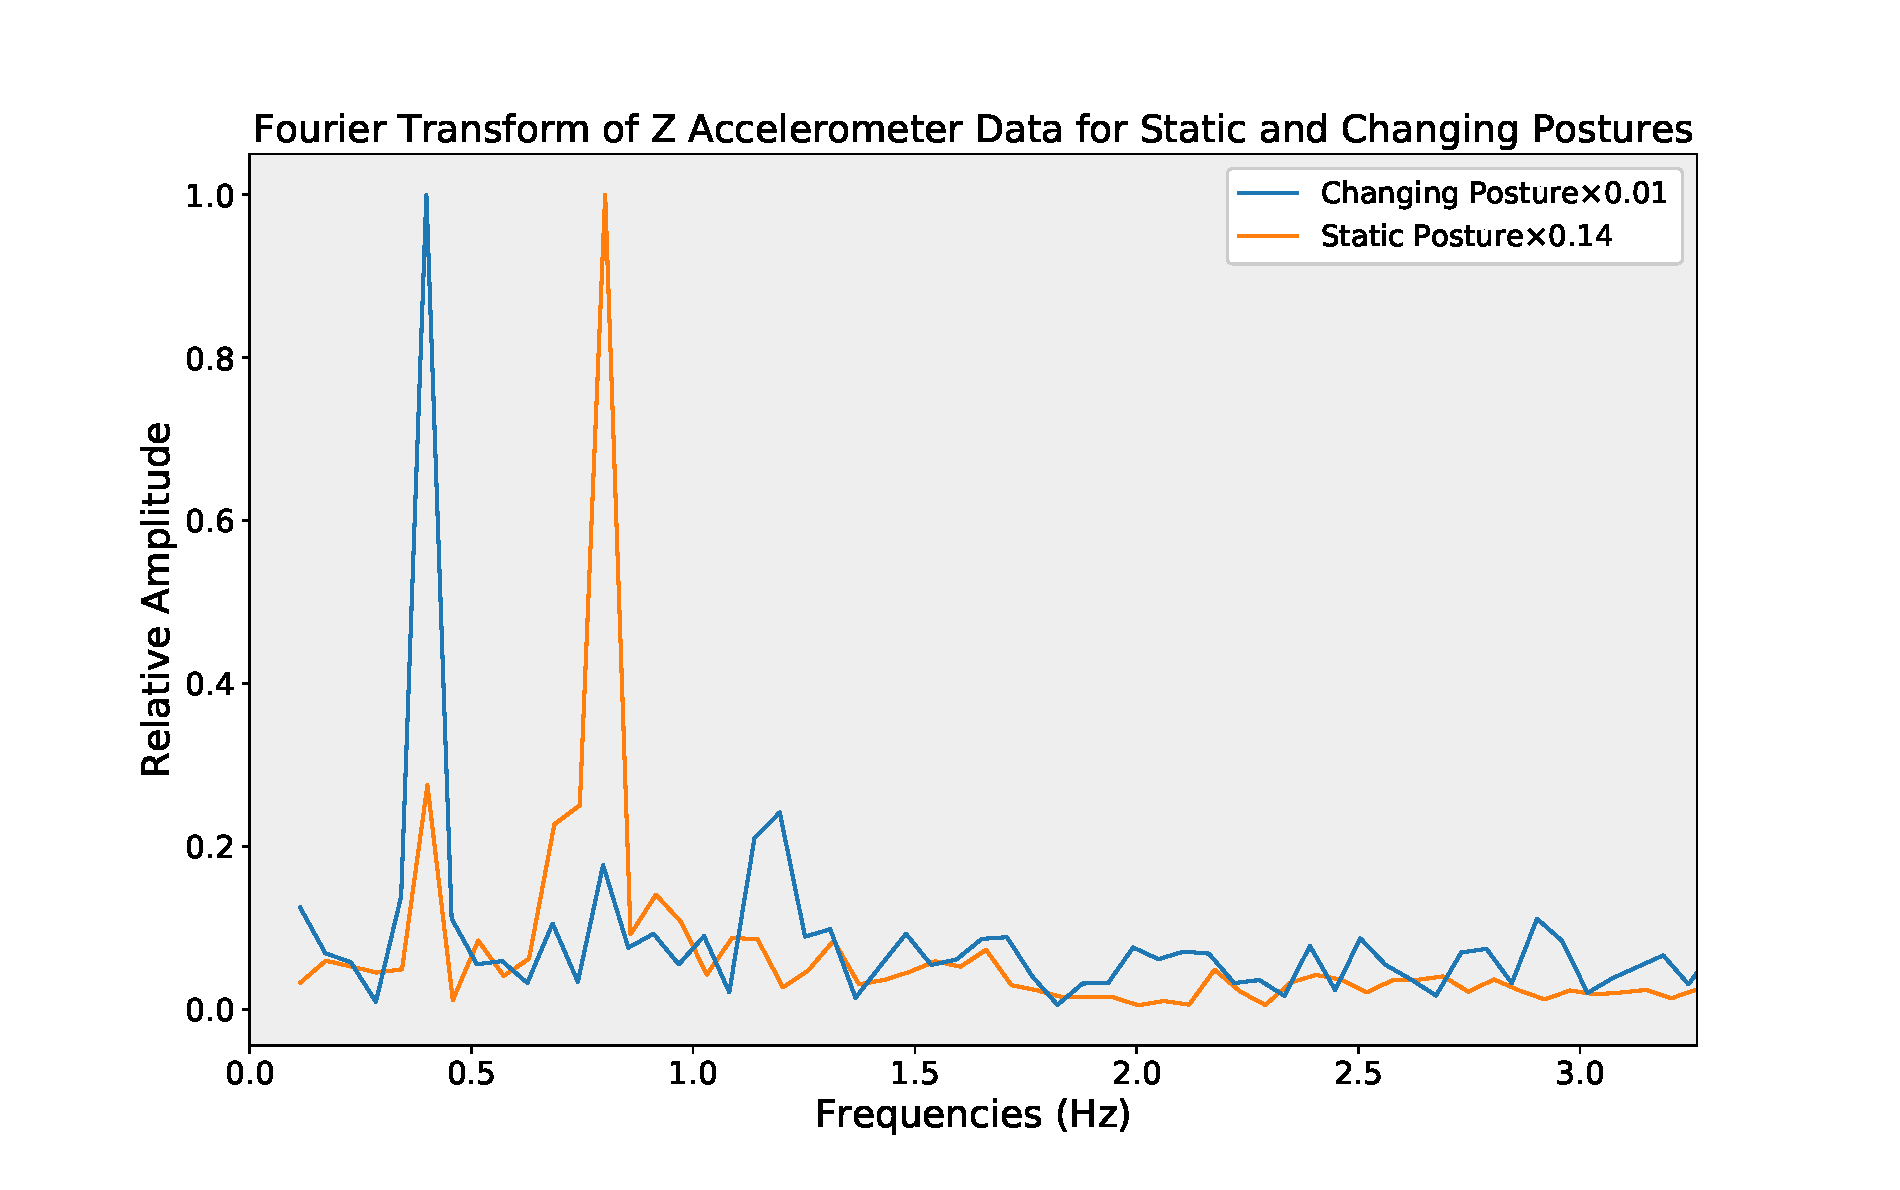
\includegraphics[width=1.0\textwidth]{FrequencyDecomposition.eps}}
    \end{figure}

To select only the frequency associated with the swing, the accelerometer data was passed through a band-pass filter, with a lowcut frequency of $0.30$Hz, and a highcut frequency of $0.50$Hz. With only the frequency of the swing selected the resulting curve can be inverted, and an offset can be added such that the final curve resembles that of the large encoder values, this process is shown in figure \ref{fig:AccelerometerFiltering}. This method of filtering allows the Z accelerometer data to be 'converted' to the large encoder value, the magnitude of the curve sinusodial motion is unimportant, as it is only the time at which the peaks occur that is used each of the previous timing methods. This means that the filtered Z accelerometer data can be used as a direct substitute for the large encoder value such that no modifications need to be made to any of the timing methods.\\

    \begin{figure}[!htb]
        \centering
        \captionbox
             {Z accelerometer values are first passed through a bandpass filter, subsequently the values are flipped and offset to recreate large encoder values.\label{fig:AccelerometerFiltering}}
             {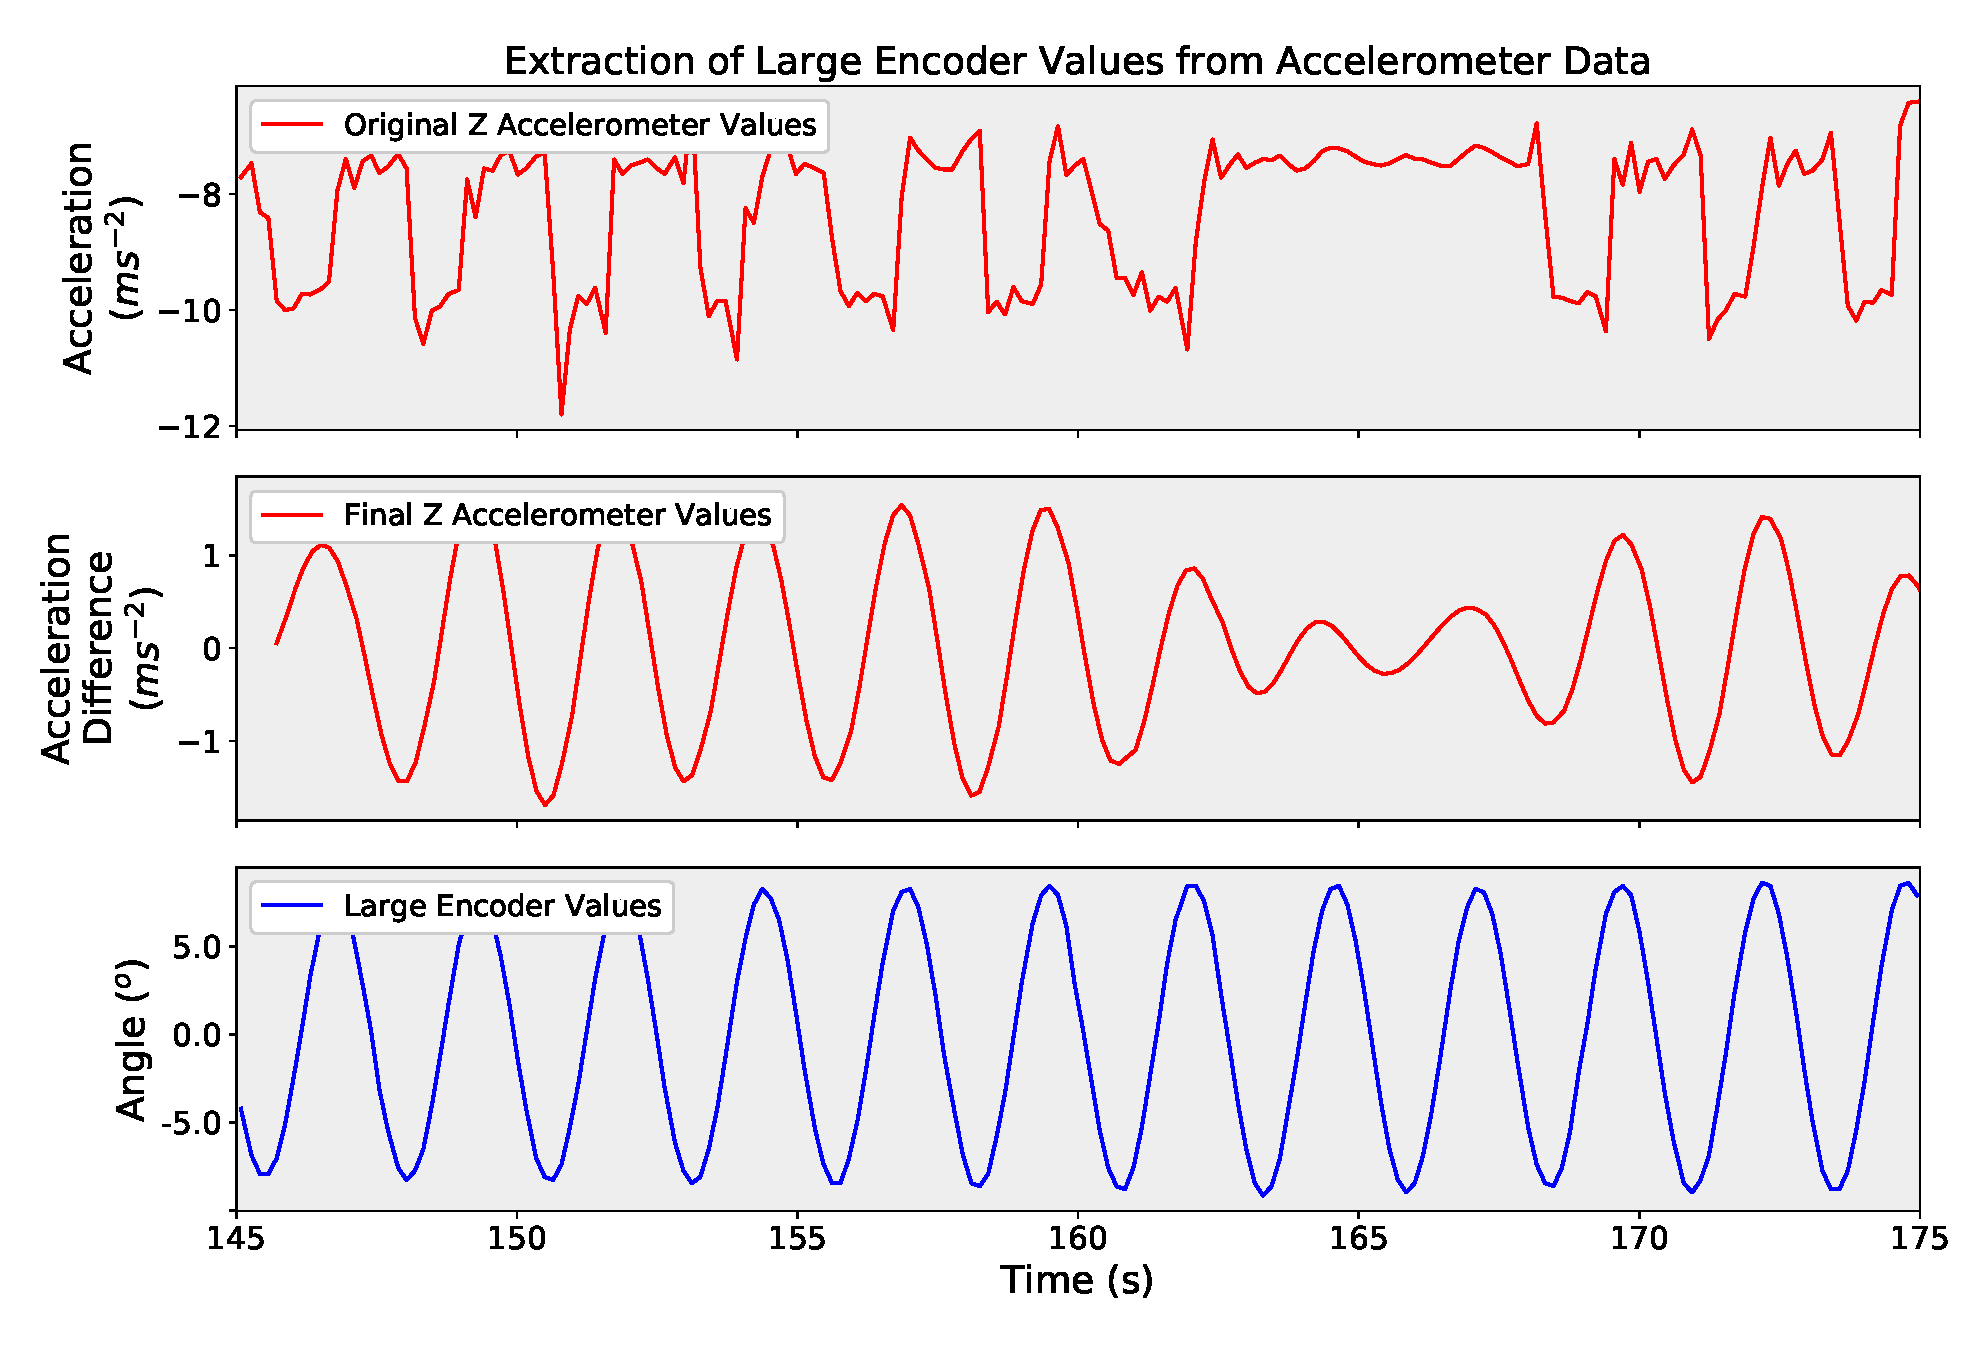
\includegraphics[width=1.0\textwidth]{AccelerometerFiltering.eps}}
    \end{figure}
    
As this algorithm doesn't change the timing of the maxima, it will be subject to the same maximum angle that the individual timing method it is connected to has. One point of interest however is the reliability in making this conversion from accelerometer to equivalent large encoder value. Figure \ref{fig:PositionAccelerometer} shows a sample of this algorithm reacting in real time. This algorithm is able to switch at the correct times for the majority of cases, unfortunately however, Nao occasionally fails to transmit the correct accelerometer value, as can be seen from $(162-168)$seconds. In this case the algorithm is unable to adapt and will not kick. The reason for this recording error is unknown due to time restrictions.\\

    \begin{figure}[!htb]
        \centering
        \captionbox
             {Response of algorithm to Z accelerometer data, doesn't react when poor values are recorded.\label{fig:PositionAccelerometer}}
             {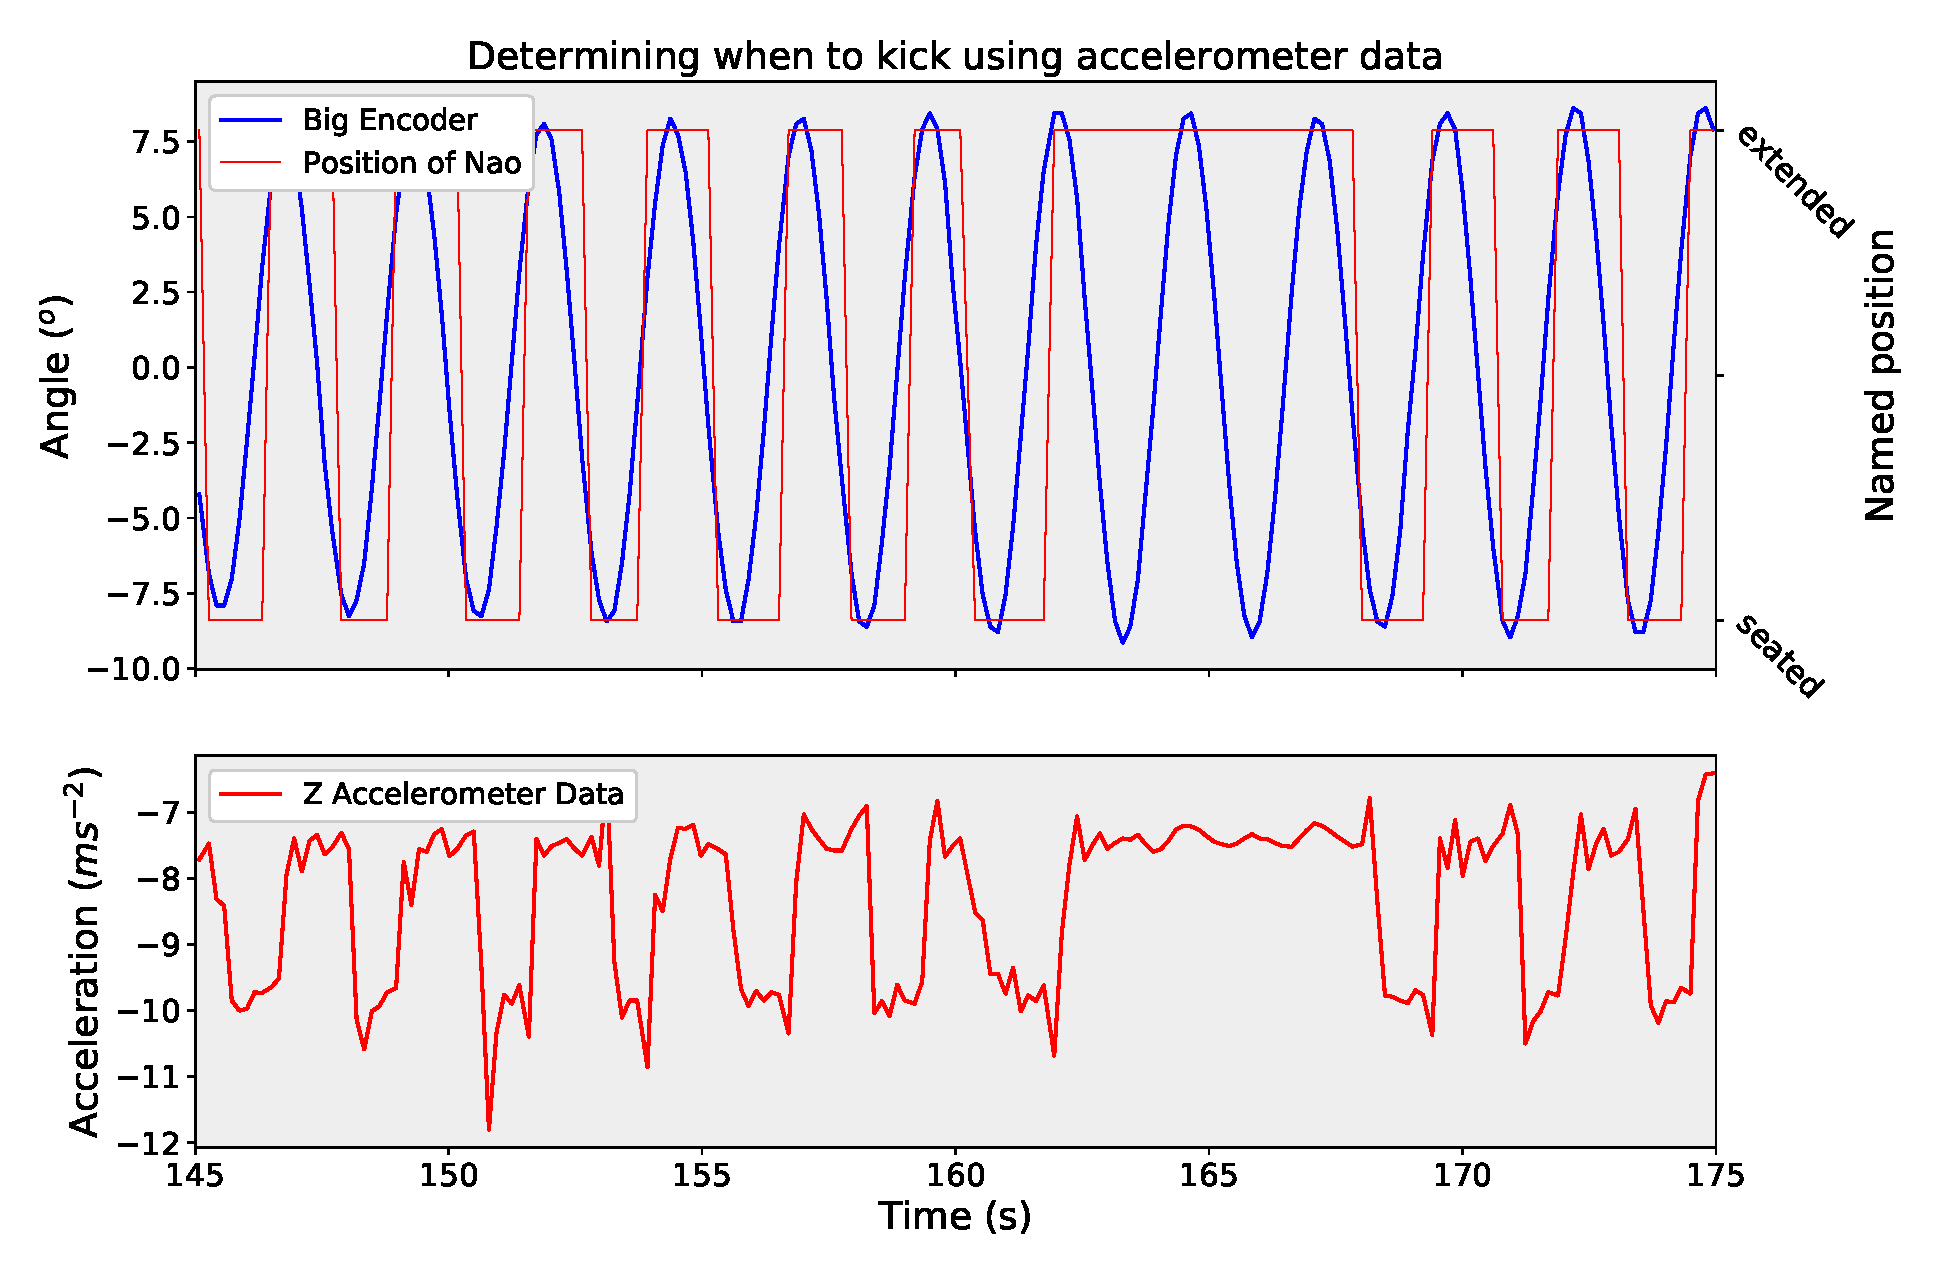
\includegraphics[width=1.0\textwidth]{PositionAccelerometer.eps}}
    \end{figure}
    
It is worth noting that the implementation of this algorithm as it currently stands hinges entirely on the asymmetry of the positions. This is a poor method to use and the proper way to implement this would be by extracting the $0.8$Hz frequency corresponding to the accelerometer data, then halving the frequency of the signal and using this as the substitute for the large encoder value.

\clearpage


\section{Double Pendulum}
\subsection{Start-up}
\ruleline{James Doering}
How is this different to the single pendulum version? Need data on low angle oscillations. How should tactics change?

\subsection{Adjusting Algorithms}\label{sec:AdjustingAlgorithms}
\ruleline{George Sheppard}
To adjust for the new setup of the swing, the single pendulum algorithms needed to be adjusted such that they would account for the motion of the swing below the hinges. For this reason a new coordinate system was defined that took into account the angle of the small encoders. This new coordinate system was defined by an angle named the 'total angle', and a diagram of this angle is shown in figure \ref{fig:TotalAngleDiagram}. The large encoder value used previously in all single pendulum algorithms was then replaced with this new total angle to create the new algorithms.

    \begin{figure}[!htb]
        \centering
        \captionbox
             {Adjustment made to the angle used in calculating the maximas, for single and double pendulum.\label{fig:TotalAngleDiagram}}
             {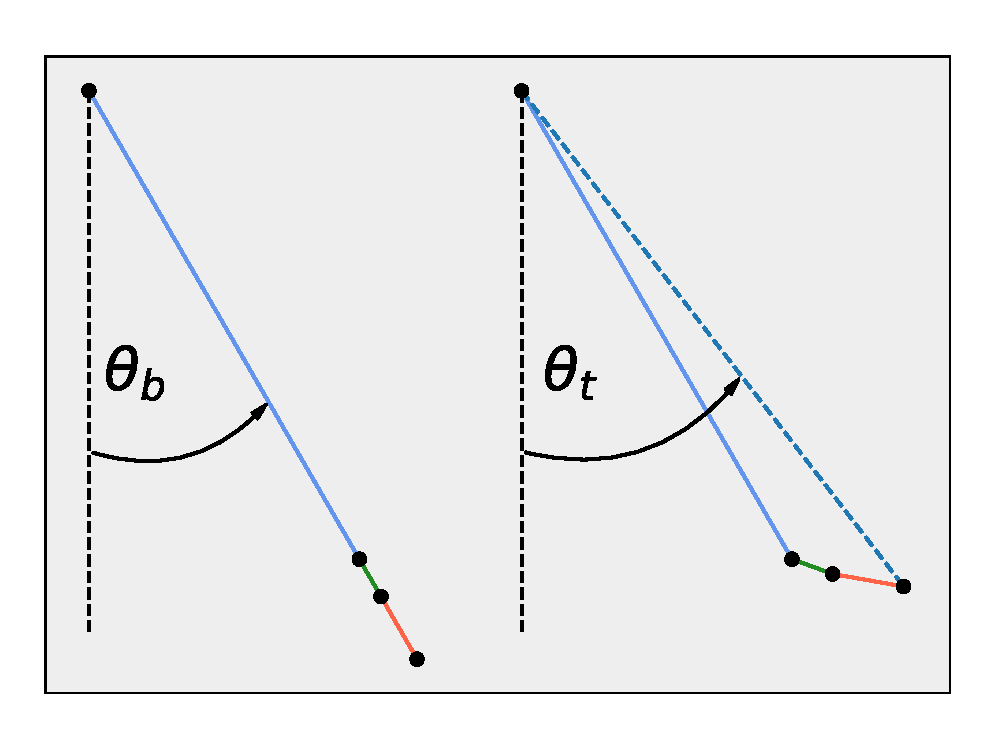
\includegraphics[width=1.0\textwidth]{TotalAngleDiagram.eps}}
    \end{figure}
    
\clearpage

\subsection{Increasing QP Rotational}
From initial experimentation with the double pendulum, it was found that the period of the motion depended largely on the specific motion of the swing below the first now opened hinge. This motion is large when Nao implements the rotational motion seen in section \ref{sec:Increasing QP Rotational}, and as such the angular velocity timing method was decided to be optimum for a rotational motion, as the quarter period was difficult to determine and varied a large amount.\\

The adjusted angular velocity based on the total angle was used to decide when Nao has reached the maximum of his swing. For an efficient motion, the speed of Nao's motion had to be reduced. This is because when Nao was switching postures at the maximum speed, the motion of the rods below the first hinge became very chaotic, and ultimately caused a reduction in the total swinging angle. By reducing the posture switching speed to half of the maximum this motion was mostly under control, such that there was mostly a smooth swing.\\

Figure \ref{fig:DoublePendulumData3} shows the results for this method. This algorithm maintains an amplitude of around $10^o$, but due to the motion below the first hinge there are large jumps in the angle of successive peaks.

    \begin{figure}[!htb]
        \centering
        \captionbox
             {Total angle reached using rotational pumping, with the alteration to the angle defined in section \ref{sec:AdjustingAlgorithms}.\label{fig:DoublePendulumData3}}
             {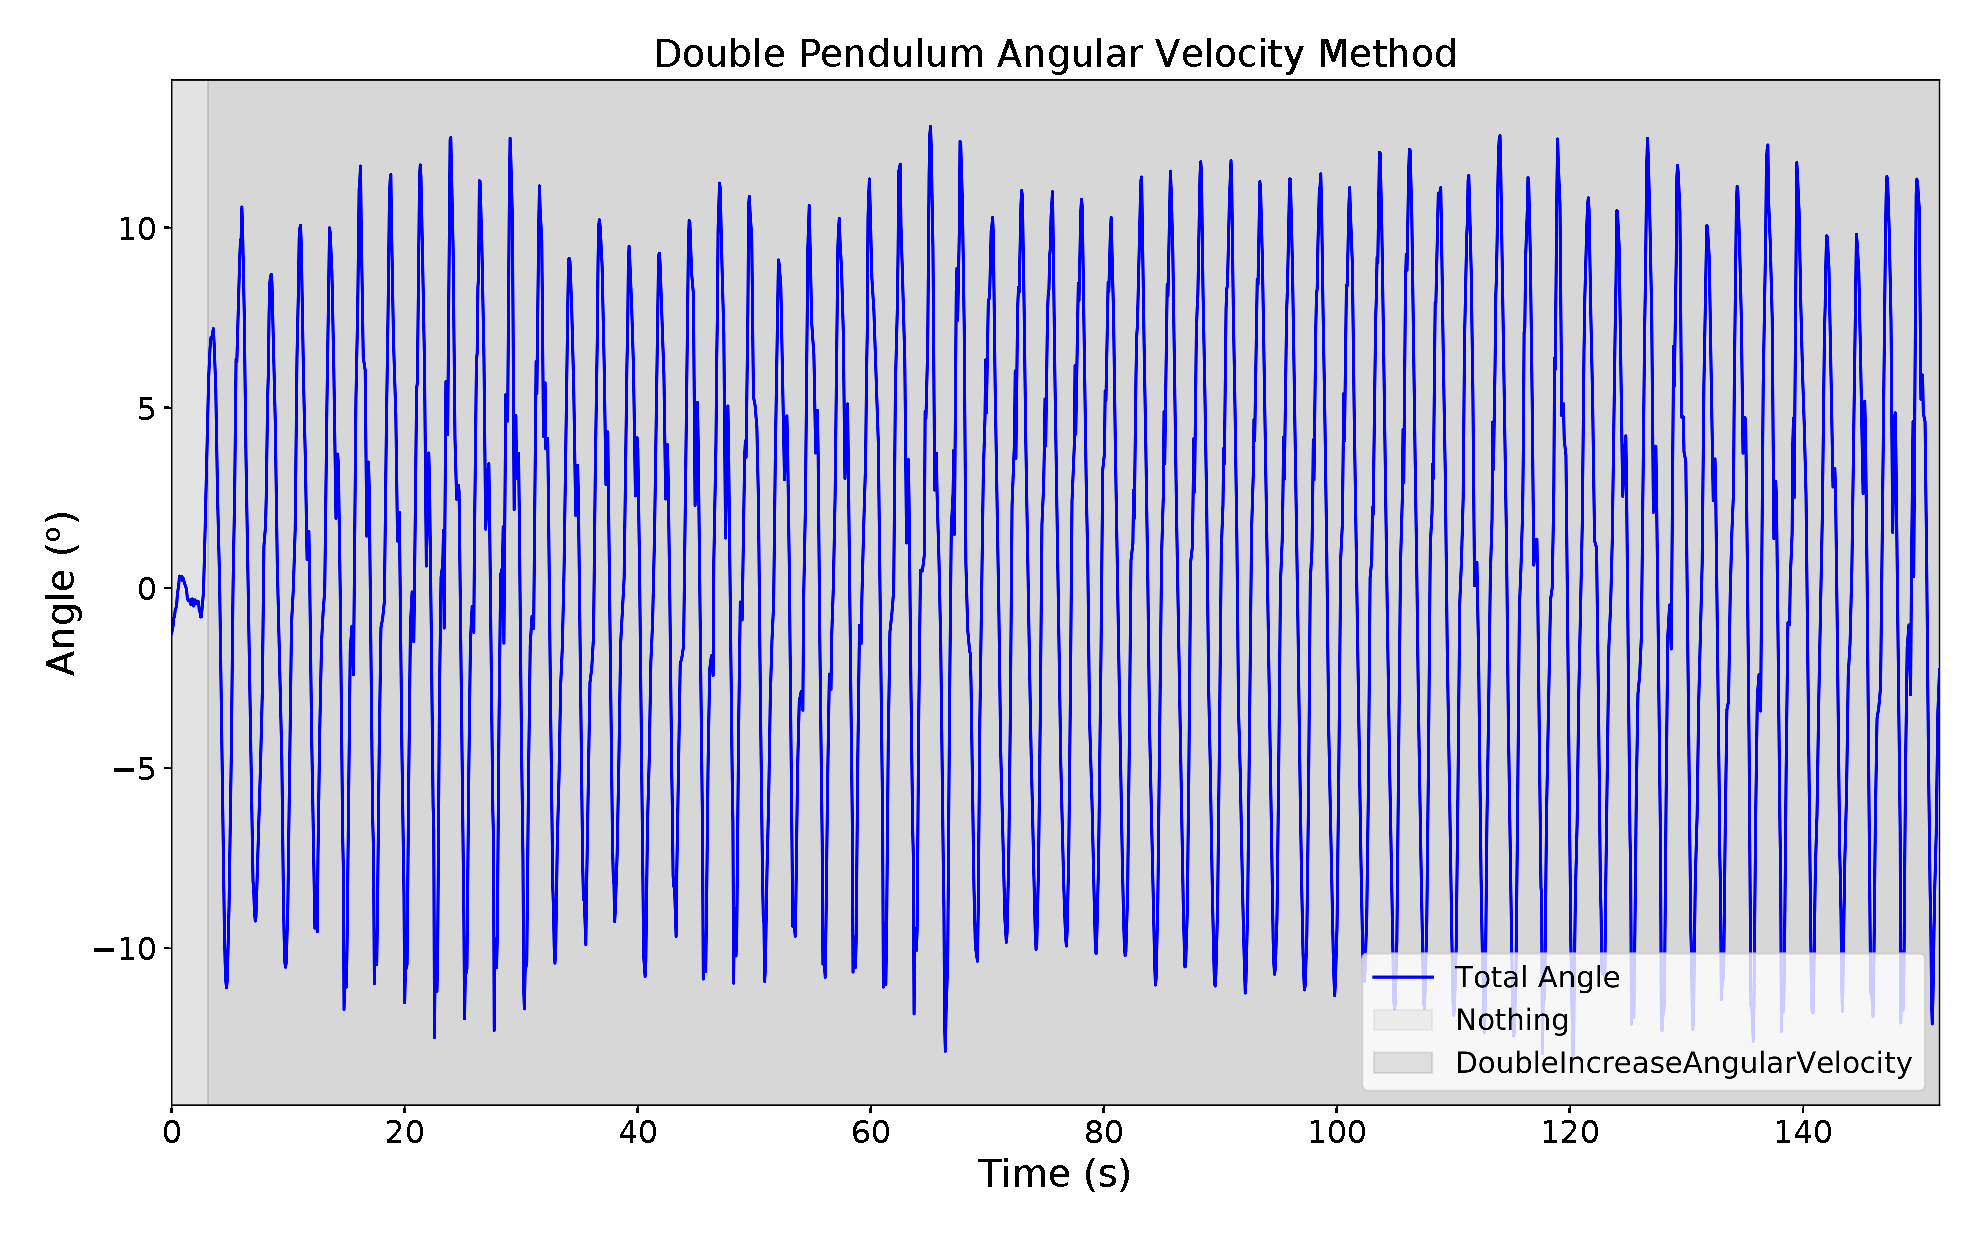
\includegraphics[width=1.0\textwidth]{DoublePendulumRotationalAngular.eps}}
    \end{figure}

\subsection{Increasing QP Parametric}

\subsection{Discussion}

\section{Future Suggestions}
\ruleline{David Thomas}
There are several ideas that given a longer amount of time we would have liked to investigate, but serve as points of interest for future years:

Improvements to the seat of the swing could be made in order to improve the stability of Nao when changing positions. During the current project, tape was required to secure Nao but with a re-milled seat, grips could be made to attach to the rear of the hips and prevent any lifting motion. A CAD designed attachment could also be made for Nao's torso and feet in order for weights to be quickly added and removed. This would allow much greater amplitudes to be reached and securing the weights to Nao's body will prevent any scratching or risk of tape becoming loose. It could also be beneficial in future projects to investigate the use of internal sensors as inputs for the machine learning teams to train their virtual robot. This could allow Nao to become be self sufficient and not rely on any external sensor inputs, such as the encoders. There has also previously been some investigation into the range of motion of Nao was compared to that of a human but this performed on a rope swing and much of the motions were unrepresentative of what Nao could achieve. It could be interesting in future years to motion track a human swinging on a rod swing, especially from a self-start point of view to see how these real life motions could be translated onto Nao. The flexible shaft on the encoder adds a lot of sideways motion to the swing, and makes it difficult to maximise energy transferred to the swing, especially in the case where all the hinges are open. 
\appendix
\section{Appendix}
\subsection{Wiki} \label{sec:wiki}
\ruleline{George Sheppard}
Throughout this project, there were a large amount of issues found when trying to connect to: Nao, Webots, and the hinge encoders etc. For this reason a wiki was created to document how to set everything up correctly. This wiki is available at: https://github.com/GeorgeSheppard/Robotics. Alongside this wiki is the final code, including how to use it, the report, and any analysis files used to create plots. Feel free to clone this repository and add to it such that there remains a comprehensive guide for each year.

\subsection{Using Webots} \label{sec:usingwebots}
\ruleline{James Doering}
Connecting to Webots using the same code used to connect to Nao is possible, though requires some tinkering. The NAOQISIM controller (available \textbf{put something here!!!}) must be installed, but can only be connected to using version 2.1.4.13 of NAOqi - the real robot requires NAOqi 1.14.5, meaning the two versions must be switched between if connection to both is required. Connection will not work with non 64-bit versions of Python 2.7. If all the correct versions are used, the simulated robot should react to all commands, though speech will be printed in the Webots console. Pausing the simulation will break this connection, and will require a restart of the simulation. Similarly, computer slowdown can cause disconnection or missed commands. It is not recommended to use Webots to test the viability of algorithms, as the simulation quickly deteriorates if the computer is not strong enough, and there is no simple way to extract hinge data from a simulated swing. \\


As described in section \ref{sec:webots}, Webots was used to find the centre of mass of Nao in each posture. Despite this being automatically calculated and displayed on the screen (when enabled), there is no simple way to extract the position of the centre of mass relative to Nao - discussion with Cyberbotics revealed that this could be achieved by creating a supervisor for Nao in C++, which was beyond the scope of this project. To get around this limitation, the centre of mass was found using the viewpoint of the camera in Webots. By placing Nao at the centre of the virtual space, the viewpoint could be "zoomed" into the centre of mass until it was large and central to the screen. By carefully considering the axes and rotation of Nao, the viewpoint's position (which is given by the Webots) could be transformed to give the relative vector between Nao's centre and its centre of mass for each position. \textbf{Rewrite.}



\subsection{Fitting Damping}\label{sec:dampingboring}
\ruleline{James Doering}

\begin{figure}[h]
    \centering
    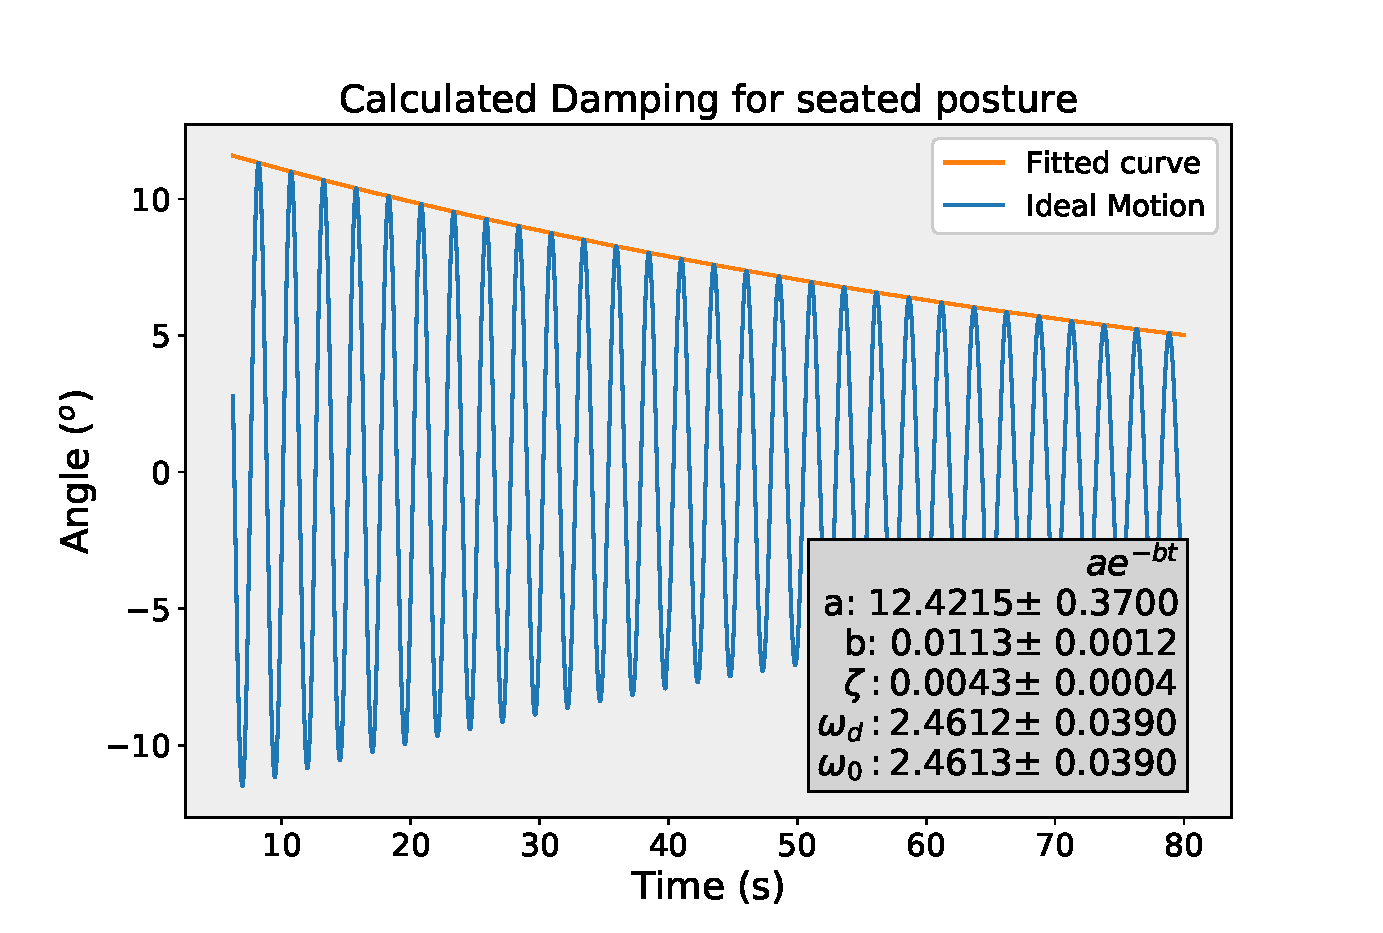
\includegraphics[width=0.6\textwidth]{SeatedDecay.eps}
    \caption{One of the eight fitted plots for the seated posture.}
    \label{fig:dampingfitexample}
\end{figure}

To obtain the plot in figure \ref{fig:dampingpositions}, where each of the posture's expected decays are compared, Nao was raised to $\approx 10^\circ$ and released. The decay of the swing was recorded for 80 seconds, with the first swing cut to remove data of Nao being lifted and dropped. The maximums of this swing were then automatically detected using SciPy's 'find\_peaks' and fitted to equation \ref{eq:damping}, producing plots similar to figure \ref{fig:dampingfitexample}. This was then repeated 8 times for each of Nao's postures, producing the results and standard deviations in table \ref{tbl:damping}. Finally, equation \ref{eq:damping} was plotted for each of the postures, using an initial $\theta_0 = 10$, giving a comparison for the expected decay of each posture.



\begin{table}[hb]
\centering
\caption{The damping coefficients for each posture.}
\label{tbl:damping}
\begin{tabular}{|l|l|l|l|l|}
\hline
                         & Extended                           & Seated                             & Raised                             & Lowered                            \\ \hline
$\theta_0$ & $13.82 \pm 0.64$      & $12.42 \pm 0.37$      & $12.46 \pm 1.03$      & $14.22 \pm 0.73$      \\ \hline
$b$                        & $0.00923 \pm 0.00068$ & $0.01133 \pm 0.00115$ & $0.01153 \pm 0.00276$ & $0.01032 \pm 0.00063$ \\ \hline
$\omega_d$ & $2.475 \pm 0.0493$    & $2.490 \pm 0.039$     & $2.488 \pm 0.030$     & $2.485 \pm 0.372$     \\ \hline
$\zeta$    & $0.00373 \pm 0.00021$ & $0.00454 \pm 0.00039$ & $0.00464 \pm 0.00112$ & $0.00416 \pm 0.00028$ \\ \hline
\end{tabular}
\end{table}

\bibliographystyle{ieeetr}
\bibliography{References}
\end{document}